\documentclass[twoside]{book}

% Packages required by doxygen
\usepackage{fixltx2e}
\usepackage{calc}
\usepackage{doxygen}
\usepackage[export]{adjustbox} % also loads graphicx
\usepackage{graphicx}
\usepackage[utf8]{inputenc}
\usepackage{makeidx}
\usepackage{multicol}
\usepackage{multirow}
\PassOptionsToPackage{warn}{textcomp}
\usepackage{textcomp}
\usepackage[nointegrals]{wasysym}
\usepackage[table]{xcolor}

% Font selection
\usepackage[T1]{fontenc}
\usepackage[scaled=.90]{helvet}
\usepackage{courier}
\usepackage{amssymb}
\usepackage{sectsty}
\renewcommand{\familydefault}{\sfdefault}
\allsectionsfont{%
  \fontseries{bc}\selectfont%
  \color{darkgray}%
}
\renewcommand{\DoxyLabelFont}{%
  \fontseries{bc}\selectfont%
  \color{darkgray}%
}
\newcommand{\+}{\discretionary{\mbox{\scriptsize$\hookleftarrow$}}{}{}}

% Page & text layout
\usepackage{geometry}
\geometry{%
  a4paper,%
  top=2.5cm,%
  bottom=2.5cm,%
  left=2.5cm,%
  right=2.5cm%
}
\tolerance=750
\hfuzz=15pt
\hbadness=750
\setlength{\emergencystretch}{15pt}
\setlength{\parindent}{0cm}
\setlength{\parskip}{3ex plus 2ex minus 2ex}
\makeatletter
\renewcommand{\paragraph}{%
  \@startsection{paragraph}{4}{0ex}{-1.0ex}{1.0ex}{%
    \normalfont\normalsize\bfseries\SS@parafont%
  }%
}
\renewcommand{\subparagraph}{%
  \@startsection{subparagraph}{5}{0ex}{-1.0ex}{1.0ex}{%
    \normalfont\normalsize\bfseries\SS@subparafont%
  }%
}
\makeatother

% Headers & footers
\usepackage{fancyhdr}
\pagestyle{fancyplain}
\fancyhead[LE]{\fancyplain{}{\bfseries\thepage}}
\fancyhead[CE]{\fancyplain{}{}}
\fancyhead[RE]{\fancyplain{}{\bfseries\leftmark}}
\fancyhead[LO]{\fancyplain{}{\bfseries\rightmark}}
\fancyhead[CO]{\fancyplain{}{}}
\fancyhead[RO]{\fancyplain{}{\bfseries\thepage}}
\fancyfoot[LE]{\fancyplain{}{}}
\fancyfoot[CE]{\fancyplain{}{}}
\fancyfoot[RE]{\fancyplain{}{\bfseries\scriptsize Generated by Doxygen }}
\fancyfoot[LO]{\fancyplain{}{\bfseries\scriptsize Generated by Doxygen }}
\fancyfoot[CO]{\fancyplain{}{}}
\fancyfoot[RO]{\fancyplain{}{}}
\renewcommand{\footrulewidth}{0.4pt}
\renewcommand{\chaptermark}[1]{%
  \markboth{#1}{}%
}
\renewcommand{\sectionmark}[1]{%
  \markright{\thesection\ #1}%
}

% Indices & bibliography
\usepackage{natbib}
\usepackage[titles]{tocloft}
\setcounter{tocdepth}{3}
\setcounter{secnumdepth}{5}
\makeindex

% Hyperlinks (required, but should be loaded last)
\usepackage{ifpdf}
\ifpdf
  \usepackage[pdftex,pagebackref=true]{hyperref}
\else
  \usepackage[ps2pdf,pagebackref=true]{hyperref}
\fi
\hypersetup{%
  colorlinks=true,%
  linkcolor=blue,%
  citecolor=blue,%
  unicode%
}

% Custom commands
\newcommand{\clearemptydoublepage}{%
  \newpage{\pagestyle{empty}\cleardoublepage}%
}

\usepackage{caption}
\captionsetup{labelsep=space,justification=centering,font={bf},singlelinecheck=off,skip=4pt,position=top}

%===== C O N T E N T S =====

\begin{document}

% Titlepage & ToC
\hypersetup{pageanchor=false,
             bookmarksnumbered=true,
             pdfencoding=unicode
            }
\pagenumbering{alph}
\begin{titlepage}
\vspace*{7cm}
\begin{center}%
{\Large My Project }\\
\vspace*{1cm}
{\large Generated by Doxygen 1.8.13}\\
\end{center}
\end{titlepage}
\clearemptydoublepage
\pagenumbering{roman}
\tableofcontents
\clearemptydoublepage
\pagenumbering{arabic}
\hypersetup{pageanchor=true}

%--- Begin generated contents ---
\chapter{Hierarchical Index}
\section{Class Hierarchy}
This inheritance list is sorted roughly, but not completely, alphabetically\+:\begin{DoxyCompactList}
\item \contentsline{section}{Automata}{\pageref{class_automata}}{}
\begin{DoxyCompactList}
\item \contentsline{section}{A\+FD}{\pageref{class_a_f_d}}{}
\item \contentsline{section}{A\+FN}{\pageref{class_a_f_n}}{}
\end{DoxyCompactList}
\item \contentsline{section}{Estado}{\pageref{class_estado}}{}
\item \contentsline{section}{Pruebas}{\pageref{class_pruebas}}{}
\begin{DoxyCompactList}
\item \contentsline{section}{Pruebas\+A\+FD}{\pageref{class_pruebas_a_f_d}}{}
\item \contentsline{section}{Pruebas\+A\+FN}{\pageref{class_pruebas_a_f_n}}{}
\end{DoxyCompactList}
\item \contentsline{section}{Subconjunto}{\pageref{class_subconjunto}}{}
\item \contentsline{section}{Transicion}{\pageref{class_transicion}}{}
\end{DoxyCompactList}

\chapter{Class Index}
\section{Class List}
Here are the classes, structs, unions and interfaces with brief descriptions\+:\begin{DoxyCompactList}
\item\contentsline{section}{\hyperlink{class_a_f_d}{A\+FD} }{\pageref{class_a_f_d}}{}
\item\contentsline{section}{\hyperlink{class_a_f_n}{A\+FN} }{\pageref{class_a_f_n}}{}
\item\contentsline{section}{\hyperlink{class_automata}{Automata} }{\pageref{class_automata}}{}
\item\contentsline{section}{\hyperlink{class_estado}{Estado} }{\pageref{class_estado}}{}
\item\contentsline{section}{\hyperlink{class_pruebas}{Pruebas} }{\pageref{class_pruebas}}{}
\item\contentsline{section}{\hyperlink{class_pruebas_a_f_d}{Pruebas\+A\+FD} }{\pageref{class_pruebas_a_f_d}}{}
\item\contentsline{section}{\hyperlink{class_pruebas_a_f_n}{Pruebas\+A\+FN} }{\pageref{class_pruebas_a_f_n}}{}
\item\contentsline{section}{\hyperlink{class_subconjunto}{Subconjunto} }{\pageref{class_subconjunto}}{}
\item\contentsline{section}{\hyperlink{class_transicion}{Transicion} }{\pageref{class_transicion}}{}
\end{DoxyCompactList}

\chapter{Class Documentation}
\hypertarget{class_a_f_d}{}\section{A\+FD Class Reference}
\label{class_a_f_d}\index{A\+FD@{A\+FD}}
Inheritance diagram for A\+FD\+:\begin{figure}[H]
\begin{center}
\leavevmode
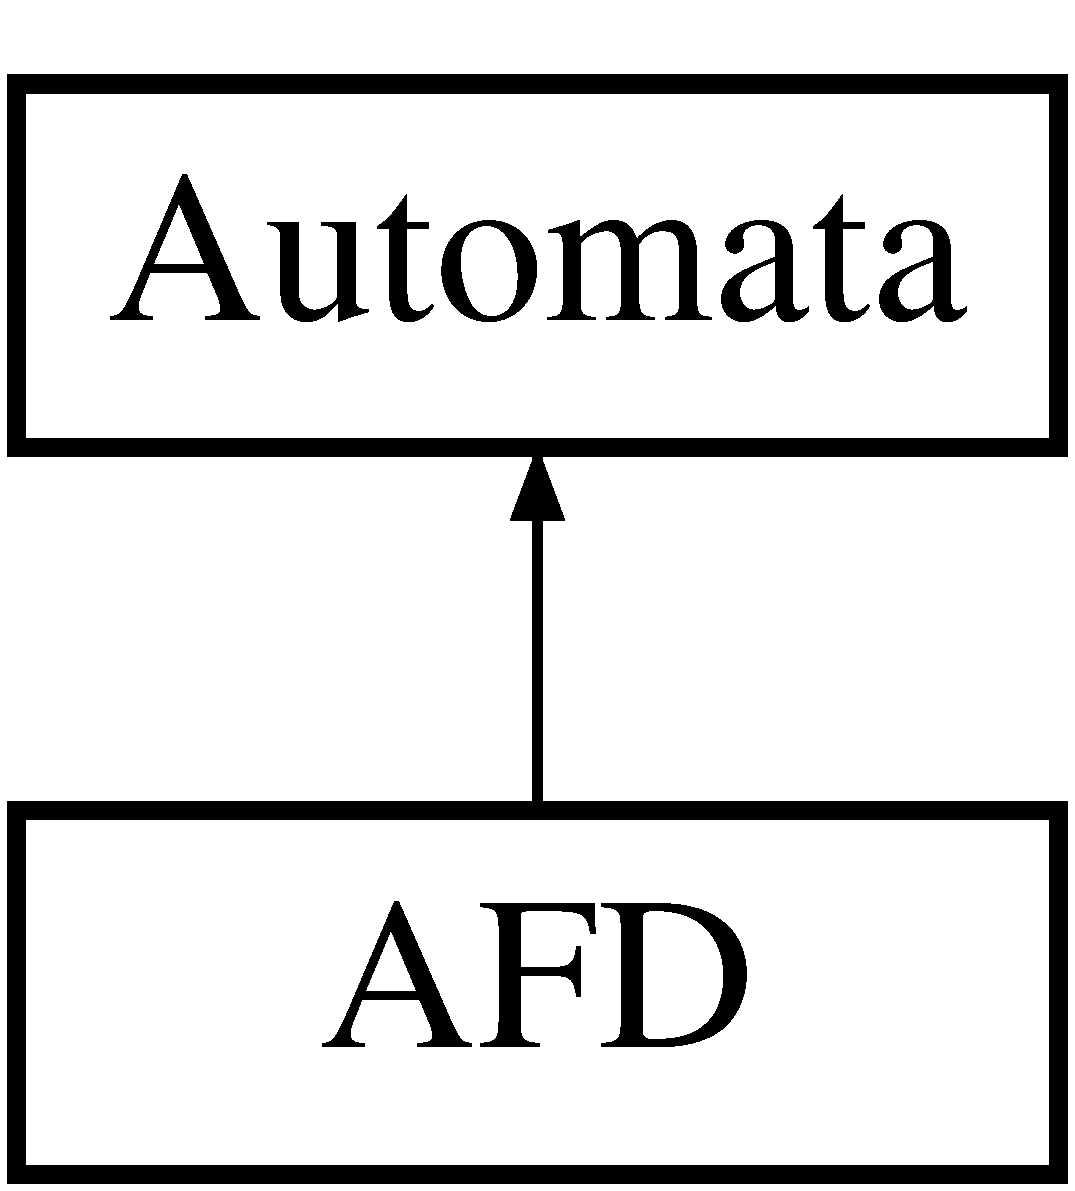
\includegraphics[height=2.000000cm]{class_a_f_d}
\end{center}
\end{figure}
\subsection*{Public Member Functions}
\begin{DoxyCompactItemize}
\item 
\mbox{\Hypertarget{class_a_f_d_a145cb15cbb67e68be849c2169bb91ad5}\label{class_a_f_d_a145cb15cbb67e68be849c2169bb91ad5}} 
{\bfseries A\+FD} (std\+::string archivo, std\+::string tipo)
\item 
\mbox{\Hypertarget{class_a_f_d_a2cf1c9284bfa3a73d44d36c2a48013f7}\label{class_a_f_d_a2cf1c9284bfa3a73d44d36c2a48013f7}} 
{\bfseries A\+FD} (std\+::vector$<$ \hyperlink{class_estado}{Estado} $\ast$$>$ estados, std\+::vector$<$ char $>$ alfabeto, \hyperlink{class_estado}{Estado} $\ast$estado\+Inicial, std\+::vector$<$ \hyperlink{class_transicion}{Transicion} $\ast$$>$ tabla\+De\+Transiciones)
\item 
bool \hyperlink{class_a_f_d_a58a86635aa33739a2b58cfa06bdd9d3d}{cambiar\+De\+Estado\+A\+FD} (std\+::vector$<$ \hyperlink{class_estado}{Estado} $\ast$$>$ estados, std\+::vector$<$ \hyperlink{class_transicion}{Transicion} $\ast$$>$ tabla\+De\+Transiciones, \hyperlink{class_estado}{Estado} $\ast$estado\+Actual, std\+::string cadena, char simbolo, int indice)
\end{DoxyCompactItemize}
\subsection*{Additional Inherited Members}


\subsection{Member Function Documentation}
\mbox{\Hypertarget{class_a_f_d_a58a86635aa33739a2b58cfa06bdd9d3d}\label{class_a_f_d_a58a86635aa33739a2b58cfa06bdd9d3d}} 
\index{A\+FD@{A\+FD}!cambiar\+De\+Estado\+A\+FD@{cambiar\+De\+Estado\+A\+FD}}
\index{cambiar\+De\+Estado\+A\+FD@{cambiar\+De\+Estado\+A\+FD}!A\+FD@{A\+FD}}
\subsubsection{\texorpdfstring{cambiar\+De\+Estado\+A\+F\+D()}{cambiarDeEstadoAFD()}}
{\footnotesize\ttfamily bool A\+F\+D\+::cambiar\+De\+Estado\+A\+FD (\begin{DoxyParamCaption}\item[{std\+::vector$<$ \hyperlink{class_estado}{Estado} $\ast$$>$}]{estados,  }\item[{std\+::vector$<$ \hyperlink{class_transicion}{Transicion} $\ast$$>$}]{tabla\+De\+Transiciones,  }\item[{\hyperlink{class_estado}{Estado} $\ast$}]{estado\+Actual,  }\item[{std\+::string}]{cadena,  }\item[{char}]{simbolo,  }\item[{int}]{indice }\end{DoxyParamCaption})}

Esta función realiza el cambio de estados (funcion de transicion), de un \hyperlink{class_a_f_d}{A\+FD} Recibe\+: -\/vector$<$Estado$\ast$$>$ estados \+:\+: vector de estados del \hyperlink{class_a_f_d}{A\+FD} -\/vector$<$Transicion$\ast$$>$ tabla\+De\+Transiciones \+:\+: tabla de transiciones del \hyperlink{class_a_f_d}{A\+FD} -\/\+Estado$\ast$ estado\+Actual \+:\+: El estado en el que se encuentra. -\/string cadena \+:\+: La cadena a evaluar -\/char simbolo \+:\+: El simbolo de transicion -\/int indice \+:\+: La posicion actual de la cadena Regresa\+: -\/true \+:\+: Si la cadena fue validada -\/false \+:\+: Si la cadena no fue validada 

The documentation for this class was generated from the following files\+:\begin{DoxyCompactItemize}
\item 
A\+F\+D.\+hpp\item 
A\+F\+D.\+cpp\end{DoxyCompactItemize}

\hypertarget{class_a_f_n}{}\section{A\+FN Class Reference}
\label{class_a_f_n}\index{A\+FN@{A\+FN}}
Inheritance diagram for A\+FN\+:\begin{figure}[H]
\begin{center}
\leavevmode
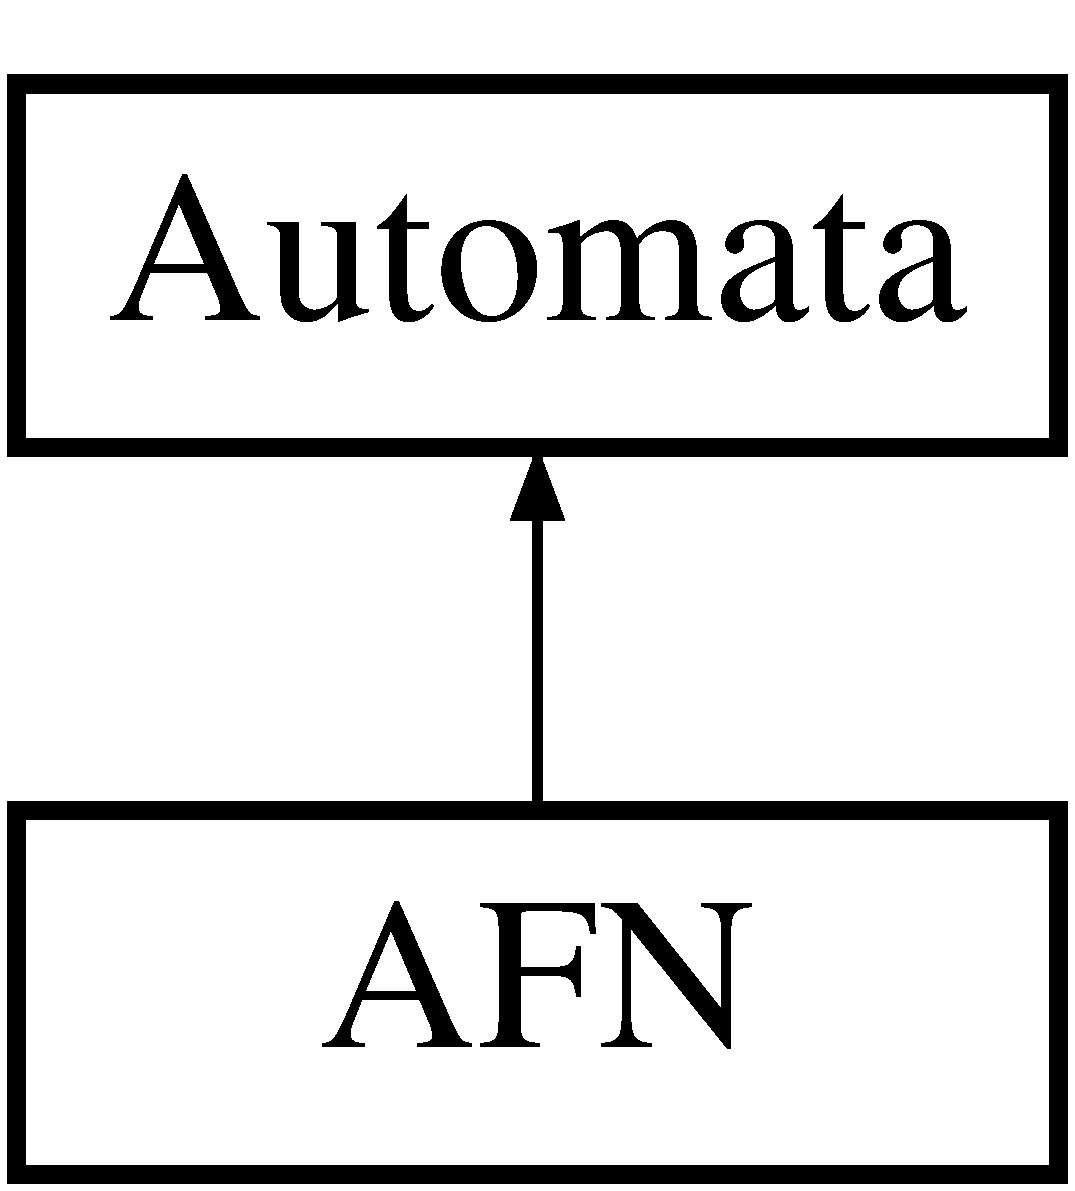
\includegraphics[height=2.000000cm]{class_a_f_n}
\end{center}
\end{figure}
\subsection*{Public Member Functions}
\begin{DoxyCompactItemize}
\item 
\mbox{\Hypertarget{class_a_f_n_a1a1a5a306993dc75210534dc44d68b6e}\label{class_a_f_n_a1a1a5a306993dc75210534dc44d68b6e}} 
{\bfseries A\+FN} (std\+::string archivo, std\+::string tipo)
\item 
\mbox{\Hypertarget{class_a_f_n_a91830f0864d932083dd22fdd37130ccf}\label{class_a_f_n_a91830f0864d932083dd22fdd37130ccf}} 
{\bfseries A\+FN} (std\+::vector$<$ \hyperlink{class_estado}{Estado} $\ast$$>$ estados, std\+::vector$<$ char $>$ alfabeto, \hyperlink{class_estado}{Estado} $\ast$estado\+Inicial, std\+::vector$<$ \hyperlink{class_transicion}{Transicion} $\ast$$>$ tabla\+De\+Transiciones)
\item 
\mbox{\Hypertarget{class_a_f_n_a6182f3845980b55ce144e89a3e5f0d1d}\label{class_a_f_n_a6182f3845980b55ce144e89a3e5f0d1d}} 
{\bfseries A\+FN} (std\+::vector$<$ \hyperlink{class_estado}{Estado} $\ast$$>$ estados, std\+::vector$<$ char $>$ alfabeto, \hyperlink{class_estado}{Estado} $\ast$estado\+Inicial, \hyperlink{class_estado}{Estado} $\ast$estado\+Final, std\+::vector$<$ \hyperlink{class_transicion}{Transicion} $\ast$$>$ tabla\+De\+Transiciones)
\item 
bool \hyperlink{class_a_f_n_afb6a2f99f54906074bd00e49538ea1f7}{cambiar\+De\+Estado\+A\+FN} (std\+::vector$<$ \hyperlink{class_estado}{Estado} $\ast$$>$ estados, std\+::vector$<$ \hyperlink{class_transicion}{Transicion} $\ast$$>$ tabla\+De\+Transiciones, \hyperlink{class_estado}{Estado} $\ast$estado\+Actual, std\+::string cadena, char simbolo, int indice)
\item 
void \hyperlink{class_a_f_n_a3722c00ec07a1df9887336a48ce33050}{renumerar\+Estados} (\hyperlink{class_a_f_n}{A\+FN} $\ast$subafn, int numero)
\item 
bool \hyperlink{class_a_f_n_a8435129e1a74e46b2727ddc087b7b3eb}{buscar\+En\+Alfabeto} (\hyperlink{class_a_f_n}{A\+FN} $\ast$afn, char c)
\item 
void \hyperlink{class_a_f_n_ac4e76a6828f9e227ed460d2e75a3a965}{agregar\+Simbolo\+Al\+Alfabeto} (\hyperlink{class_a_f_n}{A\+FN} $\ast$afn, char c)
\item 
void \hyperlink{class_a_f_n_a1c17f6a2dd580162303127bfbdac2d4b}{copiar\+Alfabeto} (\hyperlink{class_a_f_n}{A\+FN} $\ast$afn, \hyperlink{class_a_f_n}{A\+FN} subafn)
\item 
void \hyperlink{class_a_f_n_aaf3c4c74bdc3bc0bc31c1513773fbce2}{agregar\+Transicion} (\hyperlink{class_a_f_n}{A\+FN} $\ast$afn, int estado1, int estado2, char simbolo, bool es\+Epsilon)
\item 
void \hyperlink{class_a_f_n_a67852dd0b85a91d9114df429592850ac}{agregar\+Transicion\+Epsilon} (\hyperlink{class_a_f_n}{A\+FN} $\ast$afn, \hyperlink{class_estado}{Estado} $\ast$estado1, \hyperlink{class_estado}{Estado} $\ast$estado2)
\item 
void \hyperlink{class_a_f_n_aec249b192efe9df63c9e6df4ef5b96af}{agregar\+Transiciones} (\hyperlink{class_a_f_n}{A\+FN} $\ast$afn, std\+::vector$<$ \hyperlink{class_transicion}{Transicion} $\ast$$>$ tabla\+De\+Transiciones)
\item 
void \hyperlink{class_a_f_n_a565f890649af177b45ad4111ad0d14ec}{agregar\+Estados} (\hyperlink{class_a_f_n}{A\+FN} $\ast$afn, std\+::vector$<$ \hyperlink{class_estado}{Estado} $\ast$$>$ estados)
\item 
void \hyperlink{class_a_f_n_a9585f1a106bc12c61682025cf3bce1f7}{eliminar\+Estado\+Final} (\hyperlink{class_a_f_n}{A\+FN} $\ast$afn)
\item 
void \hyperlink{class_a_f_n_a13782c7d882786a73b35e289d75c9c61}{eliminar\+Estado\+Inicial} (\hyperlink{class_a_f_n}{A\+FN} $\ast$afn)
\item 
void \hyperlink{class_a_f_n_a88e43b61c88b0fa50babdc343b432166}{modificar\+Transiciones} (\hyperlink{class_a_f_n}{A\+FN} $\ast$afn, int antiguo, int nuevo)
\item 
void \hyperlink{class_a_f_n_af2804ad2f92e4a909fd9afffb64a47c4}{swap\+Transiciones} (\hyperlink{class_a_f_n}{A\+FN} $\ast$afn, int antiguo, int nuevo)
\item 
void \hyperlink{class_a_f_n_aae3289b516c0cbf17759c279f1544e09}{renumerar\+Estado} (\hyperlink{class_a_f_n}{A\+FN} $\ast$afn, int antiguo, int nuevo)
\item 
void \hyperlink{class_a_f_n_a5247562556a165a9eae8524143ace7db}{concatenar} (\hyperlink{class_a_f_n}{A\+FN} $\ast$afn, char simbolo, bool es\+Epsilon)
\item 
void \hyperlink{class_a_f_n_ac4100292cd0b27797b1e4ee50266a079}{unir} (\hyperlink{class_a_f_n}{A\+FN} $\ast$afn, \hyperlink{class_a_f_n}{A\+FN} subafn)
\item 
void \hyperlink{class_a_f_n_a778ea064155d383463cabd37ac301a14}{aplicar\+Cerradura\+Kleen\+A\+FN} (\hyperlink{class_a_f_n}{A\+FN} $\ast$afn)
\item 
void \hyperlink{class_a_f_n_aed4763d61a7630ff6c4810be588c6089}{aplicar\+Cerradura\+Kleen} (\hyperlink{class_a_f_n}{A\+FN} $\ast$afn, char c, bool es\+Epsilon)
\item 
void \hyperlink{class_a_f_n_a951fb01c6437c633311aa15b1246a290}{aplicar\+Cerradura\+Positiva\+A\+FN} (\hyperlink{class_a_f_n}{A\+FN} $\ast$afn)
\item 
void \hyperlink{class_a_f_n_a7341086a00410a1a6a2ba4262a10d249}{aplicar\+Cerradura\+Positiva} (\hyperlink{class_a_f_n}{A\+FN} $\ast$afn, char c, bool es\+Epsilon)
\item 
void \hyperlink{class_a_f_n_a12af101cefe7072f22f9bd52442c4167}{generar\+Archivo\+A\+FN} (\hyperlink{class_a_f_n}{A\+FN} afn)
\item 
\hyperlink{class_estado}{Estado} $\ast$ \hyperlink{class_a_f_n_af6cb39f268a7722d65452b790349211d}{obtener\+Estado} (int numero\+De\+Estado)
\item 
\mbox{\Hypertarget{class_a_f_n_afa47c783d422d46161fe02266f65c861}\label{class_a_f_n_afa47c783d422d46161fe02266f65c861}} 
std\+::vector$<$ char $>$ {\bfseries obtener\+Alfabeto} ()
\end{DoxyCompactItemize}
\subsection*{Additional Inherited Members}


\subsection{Member Function Documentation}
\mbox{\Hypertarget{class_a_f_n_a565f890649af177b45ad4111ad0d14ec}\label{class_a_f_n_a565f890649af177b45ad4111ad0d14ec}} 
\index{A\+FN@{A\+FN}!agregar\+Estados@{agregar\+Estados}}
\index{agregar\+Estados@{agregar\+Estados}!A\+FN@{A\+FN}}
\subsubsection{\texorpdfstring{agregar\+Estados()}{agregarEstados()}}
{\footnotesize\ttfamily void A\+F\+N\+::agregar\+Estados (\begin{DoxyParamCaption}\item[{\hyperlink{class_a_f_n}{A\+FN} $\ast$}]{afn,  }\item[{std\+::vector$<$ \hyperlink{class_estado}{Estado} $\ast$$>$}]{estados }\end{DoxyParamCaption})}

Esta funcion agrega los elementos de un vector de estados a el automata \hyperlink{class_a_f_n}{A\+FN}. Recibe\+:
\begin{DoxyItemize}
\item A\+F\+N$\ast$ afn \+:\+: El automata \hyperlink{class_a_f_n}{A\+FN}
\item vector$<$\+Estado$\ast$$>$ estados \+:\+: El vector de estados 
\end{DoxyItemize}\mbox{\Hypertarget{class_a_f_n_ac4e76a6828f9e227ed460d2e75a3a965}\label{class_a_f_n_ac4e76a6828f9e227ed460d2e75a3a965}} 
\index{A\+FN@{A\+FN}!agregar\+Simbolo\+Al\+Alfabeto@{agregar\+Simbolo\+Al\+Alfabeto}}
\index{agregar\+Simbolo\+Al\+Alfabeto@{agregar\+Simbolo\+Al\+Alfabeto}!A\+FN@{A\+FN}}
\subsubsection{\texorpdfstring{agregar\+Simbolo\+Al\+Alfabeto()}{agregarSimboloAlAlfabeto()}}
{\footnotesize\ttfamily void A\+F\+N\+::agregar\+Simbolo\+Al\+Alfabeto (\begin{DoxyParamCaption}\item[{\hyperlink{class_a_f_n}{A\+FN} $\ast$}]{afn,  }\item[{char}]{c }\end{DoxyParamCaption})}

Esta funcion agrega un simbolo al alfabeto del automata \hyperlink{class_a_f_n}{A\+FN} Recibe\+: -\/\+A\+FN $\ast$ afn \+:\+: El automata \hyperlink{class_a_f_n}{A\+FN}
\begin{DoxyItemize}
\item char c \+:\+: El caracter a a agregar en el alfabeto 
\end{DoxyItemize}\mbox{\Hypertarget{class_a_f_n_aaf3c4c74bdc3bc0bc31c1513773fbce2}\label{class_a_f_n_aaf3c4c74bdc3bc0bc31c1513773fbce2}} 
\index{A\+FN@{A\+FN}!agregar\+Transicion@{agregar\+Transicion}}
\index{agregar\+Transicion@{agregar\+Transicion}!A\+FN@{A\+FN}}
\subsubsection{\texorpdfstring{agregar\+Transicion()}{agregarTransicion()}}
{\footnotesize\ttfamily void A\+F\+N\+::agregar\+Transicion (\begin{DoxyParamCaption}\item[{\hyperlink{class_a_f_n}{A\+FN} $\ast$}]{afn,  }\item[{int}]{estado1,  }\item[{int}]{estado2,  }\item[{char}]{simbolo,  }\item[{bool}]{es\+Epsilon }\end{DoxyParamCaption})}

Esta funcion agrega una transicion en la tabla del transiciones del \hyperlink{class_a_f_n}{A\+FN} Recibe\+:
\begin{DoxyItemize}
\item A\+F\+N$\ast$ afn \+:\+: El automata \hyperlink{class_a_f_n}{A\+FN}
\end{DoxyItemize}

int estado1 \+:\+: El estado desde el que inicia la transicion
\begin{DoxyItemize}
\item int estado2 \+:\+: El estado al que se transita
\item char simbolo \+:\+: El simbolo con el que se transita
\item bool es\+Epsilon \+:\+: Bandera para saber si la transicion es epsilon 
\end{DoxyItemize}\mbox{\Hypertarget{class_a_f_n_a67852dd0b85a91d9114df429592850ac}\label{class_a_f_n_a67852dd0b85a91d9114df429592850ac}} 
\index{A\+FN@{A\+FN}!agregar\+Transicion\+Epsilon@{agregar\+Transicion\+Epsilon}}
\index{agregar\+Transicion\+Epsilon@{agregar\+Transicion\+Epsilon}!A\+FN@{A\+FN}}
\subsubsection{\texorpdfstring{agregar\+Transicion\+Epsilon()}{agregarTransicionEpsilon()}}
{\footnotesize\ttfamily void A\+F\+N\+::agregar\+Transicion\+Epsilon (\begin{DoxyParamCaption}\item[{\hyperlink{class_a_f_n}{A\+FN} $\ast$}]{afn,  }\item[{\hyperlink{class_estado}{Estado} $\ast$}]{estado1,  }\item[{\hyperlink{class_estado}{Estado} $\ast$}]{estado2 }\end{DoxyParamCaption})}

Esta funcion agrega una transicion epsilon a la tabla de transiciones de un automata \hyperlink{class_a_f_n}{A\+FN}. Recibe\+:
\begin{DoxyItemize}
\item A\+F\+N$\ast$ afn \+:\+: El automata \hyperlink{class_a_f_n}{A\+FN}
\item Estado$\ast$ estado1 \+:\+: El estado donde inicia la transicion epsilon
\item Estado$\ast$ estado2 \+:\+: El estado a donde se transita con epsilon 
\end{DoxyItemize}\mbox{\Hypertarget{class_a_f_n_aec249b192efe9df63c9e6df4ef5b96af}\label{class_a_f_n_aec249b192efe9df63c9e6df4ef5b96af}} 
\index{A\+FN@{A\+FN}!agregar\+Transiciones@{agregar\+Transiciones}}
\index{agregar\+Transiciones@{agregar\+Transiciones}!A\+FN@{A\+FN}}
\subsubsection{\texorpdfstring{agregar\+Transiciones()}{agregarTransiciones()}}
{\footnotesize\ttfamily void A\+F\+N\+::agregar\+Transiciones (\begin{DoxyParamCaption}\item[{\hyperlink{class_a_f_n}{A\+FN} $\ast$}]{afn,  }\item[{std\+::vector$<$ \hyperlink{class_transicion}{Transicion} $\ast$$>$}]{tabla\+De\+Transiciones }\end{DoxyParamCaption})}

Esta funcion agrega los elementos de una tabla de transiciones a el automata \hyperlink{class_a_f_n}{A\+FN}. Recibe\+:
\begin{DoxyItemize}
\item A\+F\+N$\ast$ afn \+:\+: El automata \hyperlink{class_a_f_n}{A\+FN}
\item vector$<$\+Transicion$\ast$$>$ tabla\+De\+Transiciones \+:\+: El vector de transiciones 
\end{DoxyItemize}\mbox{\Hypertarget{class_a_f_n_aed4763d61a7630ff6c4810be588c6089}\label{class_a_f_n_aed4763d61a7630ff6c4810be588c6089}} 
\index{A\+FN@{A\+FN}!aplicar\+Cerradura\+Kleen@{aplicar\+Cerradura\+Kleen}}
\index{aplicar\+Cerradura\+Kleen@{aplicar\+Cerradura\+Kleen}!A\+FN@{A\+FN}}
\subsubsection{\texorpdfstring{aplicar\+Cerradura\+Kleen()}{aplicarCerraduraKleen()}}
{\footnotesize\ttfamily void A\+F\+N\+::aplicar\+Cerradura\+Kleen (\begin{DoxyParamCaption}\item[{\hyperlink{class_a_f_n}{A\+FN} $\ast$}]{afn,  }\item[{char}]{c,  }\item[{bool}]{es\+Epsilon }\end{DoxyParamCaption})}

Esta funcion aplica la cerradura de Kleen de un simbolo c, y se la concatena a un automata \hyperlink{class_a_f_n}{A\+FN}. Recibe\+:
\begin{DoxyItemize}
\item A\+F\+N$\ast$ afn \+:\+: El automata afn al que se le concatenará el automata que corresponde a la cerradura del simbolo.
\item char c \+:\+: El simbolo al que le corresponde la cerradura.
\item bool es\+Epsilon \+:\+: Bandera para saber si es una transicion epsilon. 
\end{DoxyItemize}\mbox{\Hypertarget{class_a_f_n_a778ea064155d383463cabd37ac301a14}\label{class_a_f_n_a778ea064155d383463cabd37ac301a14}} 
\index{A\+FN@{A\+FN}!aplicar\+Cerradura\+Kleen\+A\+FN@{aplicar\+Cerradura\+Kleen\+A\+FN}}
\index{aplicar\+Cerradura\+Kleen\+A\+FN@{aplicar\+Cerradura\+Kleen\+A\+FN}!A\+FN@{A\+FN}}
\subsubsection{\texorpdfstring{aplicar\+Cerradura\+Kleen\+A\+F\+N()}{aplicarCerraduraKleenAFN()}}
{\footnotesize\ttfamily void A\+F\+N\+::aplicar\+Cerradura\+Kleen\+A\+FN (\begin{DoxyParamCaption}\item[{\hyperlink{class_a_f_n}{A\+FN} $\ast$}]{afn }\end{DoxyParamCaption})}

Esta funcion aplica la cerradura de Kleen a un \hyperlink{class_a_f_n}{A\+FN}. Recibe\+:
\begin{DoxyItemize}
\item A\+F\+N$\ast$ afn \+:\+: El automata \hyperlink{class_a_f_n}{A\+FN} generado durante el proceso de conversion de ER a \hyperlink{class_a_f_n}{A\+FN}. 
\end{DoxyItemize}\mbox{\Hypertarget{class_a_f_n_a7341086a00410a1a6a2ba4262a10d249}\label{class_a_f_n_a7341086a00410a1a6a2ba4262a10d249}} 
\index{A\+FN@{A\+FN}!aplicar\+Cerradura\+Positiva@{aplicar\+Cerradura\+Positiva}}
\index{aplicar\+Cerradura\+Positiva@{aplicar\+Cerradura\+Positiva}!A\+FN@{A\+FN}}
\subsubsection{\texorpdfstring{aplicar\+Cerradura\+Positiva()}{aplicarCerraduraPositiva()}}
{\footnotesize\ttfamily void A\+F\+N\+::aplicar\+Cerradura\+Positiva (\begin{DoxyParamCaption}\item[{\hyperlink{class_a_f_n}{A\+FN} $\ast$}]{afn,  }\item[{char}]{c,  }\item[{bool}]{es\+Epsilon }\end{DoxyParamCaption})}

Esta funcion aplica la cerradura de positiva de un simbolo c, y se la concatena a un automata \hyperlink{class_a_f_n}{A\+FN}. Recibe\+:
\begin{DoxyItemize}
\item A\+F\+N$\ast$ afn \+:\+: El automata afn al que se le concatenará el automata que corresponde a la cerradura del simbolo.
\item char c \+:\+: El simbolo al que le corresponde la cerradura.
\item bool es\+Epsilon \+:\+: Bandera para saber si es una transicion epsilon. 
\end{DoxyItemize}\mbox{\Hypertarget{class_a_f_n_a951fb01c6437c633311aa15b1246a290}\label{class_a_f_n_a951fb01c6437c633311aa15b1246a290}} 
\index{A\+FN@{A\+FN}!aplicar\+Cerradura\+Positiva\+A\+FN@{aplicar\+Cerradura\+Positiva\+A\+FN}}
\index{aplicar\+Cerradura\+Positiva\+A\+FN@{aplicar\+Cerradura\+Positiva\+A\+FN}!A\+FN@{A\+FN}}
\subsubsection{\texorpdfstring{aplicar\+Cerradura\+Positiva\+A\+F\+N()}{aplicarCerraduraPositivaAFN()}}
{\footnotesize\ttfamily void A\+F\+N\+::aplicar\+Cerradura\+Positiva\+A\+FN (\begin{DoxyParamCaption}\item[{\hyperlink{class_a_f_n}{A\+FN} $\ast$}]{afn }\end{DoxyParamCaption})}

Esta funcion aplica la cerradura de positiva a un \hyperlink{class_a_f_n}{A\+FN}. Recibe\+:
\begin{DoxyItemize}
\item A\+F\+N$\ast$ afn \+:\+: El automata \hyperlink{class_a_f_n}{A\+FN} generado durante el proceso de conversion de ER a \hyperlink{class_a_f_n}{A\+FN}. 
\end{DoxyItemize}\mbox{\Hypertarget{class_a_f_n_a8435129e1a74e46b2727ddc087b7b3eb}\label{class_a_f_n_a8435129e1a74e46b2727ddc087b7b3eb}} 
\index{A\+FN@{A\+FN}!buscar\+En\+Alfabeto@{buscar\+En\+Alfabeto}}
\index{buscar\+En\+Alfabeto@{buscar\+En\+Alfabeto}!A\+FN@{A\+FN}}
\subsubsection{\texorpdfstring{buscar\+En\+Alfabeto()}{buscarEnAlfabeto()}}
{\footnotesize\ttfamily bool A\+F\+N\+::buscar\+En\+Alfabeto (\begin{DoxyParamCaption}\item[{\hyperlink{class_a_f_n}{A\+FN} $\ast$}]{afn,  }\item[{char}]{c }\end{DoxyParamCaption})}

Esta funcion busca un simbolo para saber si pertenece al alfabeto del automata. Recibe\+:
\begin{DoxyItemize}
\item A\+F\+N$\ast$ afn \+:\+: El automata \hyperlink{class_a_f_n}{A\+FN}
\item char c \+:\+: El simbolo a buscar en el alfabeto Regresa\+:
\end{DoxyItemize}

true \+:\+: Si se encontro el simbolo
\begin{DoxyItemize}
\item false \+:\+: si no se encontro 
\end{DoxyItemize}\mbox{\Hypertarget{class_a_f_n_afb6a2f99f54906074bd00e49538ea1f7}\label{class_a_f_n_afb6a2f99f54906074bd00e49538ea1f7}} 
\index{A\+FN@{A\+FN}!cambiar\+De\+Estado\+A\+FN@{cambiar\+De\+Estado\+A\+FN}}
\index{cambiar\+De\+Estado\+A\+FN@{cambiar\+De\+Estado\+A\+FN}!A\+FN@{A\+FN}}
\subsubsection{\texorpdfstring{cambiar\+De\+Estado\+A\+F\+N()}{cambiarDeEstadoAFN()}}
{\footnotesize\ttfamily bool A\+F\+N\+::cambiar\+De\+Estado\+A\+FN (\begin{DoxyParamCaption}\item[{std\+::vector$<$ \hyperlink{class_estado}{Estado} $\ast$$>$}]{estados,  }\item[{std\+::vector$<$ \hyperlink{class_transicion}{Transicion} $\ast$$>$}]{tabla\+De\+Transiciones,  }\item[{\hyperlink{class_estado}{Estado} $\ast$}]{estado\+Actual,  }\item[{std\+::string}]{cadena,  }\item[{char}]{simbolo,  }\item[{int}]{indice }\end{DoxyParamCaption})}

Esta función realiza el cambio de estados (funcion de transicion), de un \hyperlink{class_a_f_n}{A\+FN} Recibe\+: -\/vector$<$Estado$\ast$$>$ estados \+:\+: vector de estados del \hyperlink{class_a_f_n}{A\+FN} -\/vector$<$Transicion$\ast$$>$ tabla\+De\+Transiciones \+:\+: tabla de transiciones del \hyperlink{class_a_f_n}{A\+FN} -\/\+Estado$\ast$ estado\+Actual \+:\+: El estado en el que se encuentra. -\/string cadena \+:\+: La cadena a evaluar -\/char simbolo \+:\+: El simbolo de transicion -\/int indice \+:\+: La posicion actual de la cadena Regresa\+: -\/true \+:\+: Si la cadena fue validada -\/false \+:\+: Si la cadena no fue validada \mbox{\Hypertarget{class_a_f_n_a5247562556a165a9eae8524143ace7db}\label{class_a_f_n_a5247562556a165a9eae8524143ace7db}} 
\index{A\+FN@{A\+FN}!concatenar@{concatenar}}
\index{concatenar@{concatenar}!A\+FN@{A\+FN}}
\subsubsection{\texorpdfstring{concatenar()}{concatenar()}}
{\footnotesize\ttfamily void A\+F\+N\+::concatenar (\begin{DoxyParamCaption}\item[{\hyperlink{class_a_f_n}{A\+FN} $\ast$}]{afn,  }\item[{char}]{simbolo,  }\item[{bool}]{es\+Epsilon }\end{DoxyParamCaption})}

Esta funcion realiza la operacion de concatenacion de un simbolo de acuerdo a las construcciones de Thompson. Recibe\+:
\begin{DoxyItemize}
\item A\+F\+N$\ast$ afn \+:\+: El automata \hyperlink{class_a_f_n}{A\+FN}
\item char c \+:\+: El simbolo a concatenar
\item bool es\+Epsilon \+:\+: bandera para saber si es una transicion epsilon 
\end{DoxyItemize}\mbox{\Hypertarget{class_a_f_n_a1c17f6a2dd580162303127bfbdac2d4b}\label{class_a_f_n_a1c17f6a2dd580162303127bfbdac2d4b}} 
\index{A\+FN@{A\+FN}!copiar\+Alfabeto@{copiar\+Alfabeto}}
\index{copiar\+Alfabeto@{copiar\+Alfabeto}!A\+FN@{A\+FN}}
\subsubsection{\texorpdfstring{copiar\+Alfabeto()}{copiarAlfabeto()}}
{\footnotesize\ttfamily void A\+F\+N\+::copiar\+Alfabeto (\begin{DoxyParamCaption}\item[{\hyperlink{class_a_f_n}{A\+FN} $\ast$}]{afn,  }\item[{\hyperlink{class_a_f_n}{A\+FN}}]{subafn }\end{DoxyParamCaption})}

Esta funcion copia el alfabeto de un sub\+Afn a un afn principal. Recibe\+: -\/\+A\+F\+N$\ast$ afn \+:\+: El automata \hyperlink{class_a_f_n}{A\+FN} principal -\/\+A\+FN subafn \+:\+: El automata \hyperlink{class_a_f_n}{A\+FN} subafn \mbox{\Hypertarget{class_a_f_n_a9585f1a106bc12c61682025cf3bce1f7}\label{class_a_f_n_a9585f1a106bc12c61682025cf3bce1f7}} 
\index{A\+FN@{A\+FN}!eliminar\+Estado\+Final@{eliminar\+Estado\+Final}}
\index{eliminar\+Estado\+Final@{eliminar\+Estado\+Final}!A\+FN@{A\+FN}}
\subsubsection{\texorpdfstring{eliminar\+Estado\+Final()}{eliminarEstadoFinal()}}
{\footnotesize\ttfamily void A\+F\+N\+::eliminar\+Estado\+Final (\begin{DoxyParamCaption}\item[{\hyperlink{class_a_f_n}{A\+FN} $\ast$}]{afn }\end{DoxyParamCaption})}

Esta función cambia la propiedad \char`\"{}tipo\char`\"{} del estado final del \hyperlink{class_a_f_n}{A\+FN} a un estado no final. Recibe\+:
\begin{DoxyItemize}
\item A\+F\+N$\ast$ afn \+:\+: El automata \hyperlink{class_a_f_n}{A\+FN} 
\end{DoxyItemize}\mbox{\Hypertarget{class_a_f_n_a13782c7d882786a73b35e289d75c9c61}\label{class_a_f_n_a13782c7d882786a73b35e289d75c9c61}} 
\index{A\+FN@{A\+FN}!eliminar\+Estado\+Inicial@{eliminar\+Estado\+Inicial}}
\index{eliminar\+Estado\+Inicial@{eliminar\+Estado\+Inicial}!A\+FN@{A\+FN}}
\subsubsection{\texorpdfstring{eliminar\+Estado\+Inicial()}{eliminarEstadoInicial()}}
{\footnotesize\ttfamily void A\+F\+N\+::eliminar\+Estado\+Inicial (\begin{DoxyParamCaption}\item[{\hyperlink{class_a_f_n}{A\+FN} $\ast$}]{afn }\end{DoxyParamCaption})}

Esta funcion elimina el estado inicial de un automata \hyperlink{class_a_f_n}{A\+FN}. Recibe\+:
\begin{DoxyItemize}
\item A\+F\+N$\ast$ afn \+:\+: el automata \hyperlink{class_a_f_n}{A\+FN} 
\end{DoxyItemize}\mbox{\Hypertarget{class_a_f_n_a12af101cefe7072f22f9bd52442c4167}\label{class_a_f_n_a12af101cefe7072f22f9bd52442c4167}} 
\index{A\+FN@{A\+FN}!generar\+Archivo\+A\+FN@{generar\+Archivo\+A\+FN}}
\index{generar\+Archivo\+A\+FN@{generar\+Archivo\+A\+FN}!A\+FN@{A\+FN}}
\subsubsection{\texorpdfstring{generar\+Archivo\+A\+F\+N()}{generarArchivoAFN()}}
{\footnotesize\ttfamily void A\+F\+N\+::generar\+Archivo\+A\+FN (\begin{DoxyParamCaption}\item[{\hyperlink{class_a_f_n}{A\+FN}}]{afn }\end{DoxyParamCaption})}

Esta funcion genera un archivo que contiene la informacion del afn generado por una expresion regular mediante construcciones de Thompson. \mbox{\Hypertarget{class_a_f_n_a88e43b61c88b0fa50babdc343b432166}\label{class_a_f_n_a88e43b61c88b0fa50babdc343b432166}} 
\index{A\+FN@{A\+FN}!modificar\+Transiciones@{modificar\+Transiciones}}
\index{modificar\+Transiciones@{modificar\+Transiciones}!A\+FN@{A\+FN}}
\subsubsection{\texorpdfstring{modificar\+Transiciones()}{modificarTransiciones()}}
{\footnotesize\ttfamily void A\+F\+N\+::modificar\+Transiciones (\begin{DoxyParamCaption}\item[{\hyperlink{class_a_f_n}{A\+FN} $\ast$}]{afn,  }\item[{int}]{antiguo,  }\item[{int}]{nuevo }\end{DoxyParamCaption})}

Esta funcion modifica las transiciones que corresponden a un estado, remplazandolas por uno nuevo. Recibe\+:
\begin{DoxyItemize}
\item A\+F\+N$\ast$ afn \+:\+: El automata \hyperlink{class_a_f_n}{A\+FN}
\item int antiguo \+:\+: El numero del estado al que se le renumerarán las transiciones
\item int nuevo \+:\+: El numero de estado por el que serán remplazadas las transiciones donde se encuentre el estado antiguo. 
\end{DoxyItemize}\mbox{\Hypertarget{class_a_f_n_af6cb39f268a7722d65452b790349211d}\label{class_a_f_n_af6cb39f268a7722d65452b790349211d}} 
\index{A\+FN@{A\+FN}!obtener\+Estado@{obtener\+Estado}}
\index{obtener\+Estado@{obtener\+Estado}!A\+FN@{A\+FN}}
\subsubsection{\texorpdfstring{obtener\+Estado()}{obtenerEstado()}}
{\footnotesize\ttfamily \hyperlink{class_estado}{Estado} $\ast$ A\+F\+N\+::obtener\+Estado (\begin{DoxyParamCaption}\item[{int}]{numero\+De\+Estado }\end{DoxyParamCaption})}

Esta funcion obtiene un estado del automata \hyperlink{class_a_f_n}{A\+FN} de acuerdo al numero de estado que le correspone. Recibe\+:
\begin{DoxyItemize}
\item int numero\+De\+Estado \+:\+: el numero del estado del \hyperlink{class_a_f_n}{A\+FN} Regresa\+:
\item Estado$\ast$ automata\+\_\+estados\mbox{[}i\mbox{]} \+:\+: si se encontro dicho estado en la posicion i del vector de estados
\item Estado+ muerto \+:\+: Si no se encontro el estado 
\end{DoxyItemize}\mbox{\Hypertarget{class_a_f_n_aae3289b516c0cbf17759c279f1544e09}\label{class_a_f_n_aae3289b516c0cbf17759c279f1544e09}} 
\index{A\+FN@{A\+FN}!renumerar\+Estado@{renumerar\+Estado}}
\index{renumerar\+Estado@{renumerar\+Estado}!A\+FN@{A\+FN}}
\subsubsection{\texorpdfstring{renumerar\+Estado()}{renumerarEstado()}}
{\footnotesize\ttfamily void A\+F\+N\+::renumerar\+Estado (\begin{DoxyParamCaption}\item[{\hyperlink{class_a_f_n}{A\+FN} $\ast$}]{afn,  }\item[{int}]{antiguo,  }\item[{int}]{nuevo }\end{DoxyParamCaption})}

Esta funcion renumera un estado del automata \hyperlink{class_a_f_n}{A\+FN}. Recibe\+:
\begin{DoxyItemize}
\item A\+F\+N$\ast$ afn \+:\+: El automata \hyperlink{class_a_f_n}{A\+FN}
\item int antiguo \+:\+: El numero del estado a renumerar
\item int nuevo \+:\+: El nuevo numero del estado 
\end{DoxyItemize}\mbox{\Hypertarget{class_a_f_n_a3722c00ec07a1df9887336a48ce33050}\label{class_a_f_n_a3722c00ec07a1df9887336a48ce33050}} 
\index{A\+FN@{A\+FN}!renumerar\+Estados@{renumerar\+Estados}}
\index{renumerar\+Estados@{renumerar\+Estados}!A\+FN@{A\+FN}}
\subsubsection{\texorpdfstring{renumerar\+Estados()}{renumerarEstados()}}
{\footnotesize\ttfamily void A\+F\+N\+::renumerar\+Estados (\begin{DoxyParamCaption}\item[{\hyperlink{class_a_f_n}{A\+FN} $\ast$}]{subafn,  }\item[{int}]{numero }\end{DoxyParamCaption})}

Esta funcion renumera los estados de un automata sumandoles el numero de estados de el automata principal (Esta funcion se aplica a los sub\+Afn\textquotesingle{}s que se van generando en la funcion recursiva de conversión de ER a \hyperlink{class_a_f_n}{A\+FN}). Ademas renumera los estados en la tabla de transiciones. Recibe\+:
\begin{DoxyItemize}
\item \hyperlink{class_a_f_n}{A\+FN} $\ast$afn \+:\+: El automata \hyperlink{class_a_f_n}{A\+FN}
\item int numero \+:\+: El numero de estados del afn principal 
\end{DoxyItemize}\mbox{\Hypertarget{class_a_f_n_af2804ad2f92e4a909fd9afffb64a47c4}\label{class_a_f_n_af2804ad2f92e4a909fd9afffb64a47c4}} 
\index{A\+FN@{A\+FN}!swap\+Transiciones@{swap\+Transiciones}}
\index{swap\+Transiciones@{swap\+Transiciones}!A\+FN@{A\+FN}}
\subsubsection{\texorpdfstring{swap\+Transiciones()}{swapTransiciones()}}
{\footnotesize\ttfamily void A\+F\+N\+::swap\+Transiciones (\begin{DoxyParamCaption}\item[{\hyperlink{class_a_f_n}{A\+FN} $\ast$}]{afn,  }\item[{int}]{estado1,  }\item[{int}]{estado2 }\end{DoxyParamCaption})}

Esta función intercambia las transiciones de un estado antiguo a un estado nuevo y viceversa. Recibe\+:
\begin{DoxyItemize}
\item A\+F\+N$\ast$ afn \+:\+: el automata \hyperlink{class_a_f_n}{A\+FN}
\item int estado1 \+:\+: El estado 1 de intercambio
\item int estado2 \+:\+: El estado 2 de intercambio 
\end{DoxyItemize}\mbox{\Hypertarget{class_a_f_n_ac4100292cd0b27797b1e4ee50266a079}\label{class_a_f_n_ac4100292cd0b27797b1e4ee50266a079}} 
\index{A\+FN@{A\+FN}!unir@{unir}}
\index{unir@{unir}!A\+FN@{A\+FN}}
\subsubsection{\texorpdfstring{unir()}{unir()}}
{\footnotesize\ttfamily void A\+F\+N\+::unir (\begin{DoxyParamCaption}\item[{\hyperlink{class_a_f_n}{A\+FN} $\ast$}]{afn,  }\item[{\hyperlink{class_a_f_n}{A\+FN}}]{subafn }\end{DoxyParamCaption})}

Esta funcion realiza la operacion de union de acuerdo a las contrucciones de Thompson. Recibe\+:
\begin{DoxyItemize}
\item A\+F\+N$\ast$ afn \+:\+: El afn principal.
\item \hyperlink{class_a_f_n}{A\+FN} subafn \+:\+: el subafn 
\end{DoxyItemize}

The documentation for this class was generated from the following files\+:\begin{DoxyCompactItemize}
\item 
A\+F\+N.\+hpp\item 
A\+F\+N.\+cpp\end{DoxyCompactItemize}

\hypertarget{class_automata}{}\section{Automata Class Reference}
\label{class_automata}\index{Automata@{Automata}}
Inheritance diagram for Automata\+:\begin{figure}[H]
\begin{center}
\leavevmode
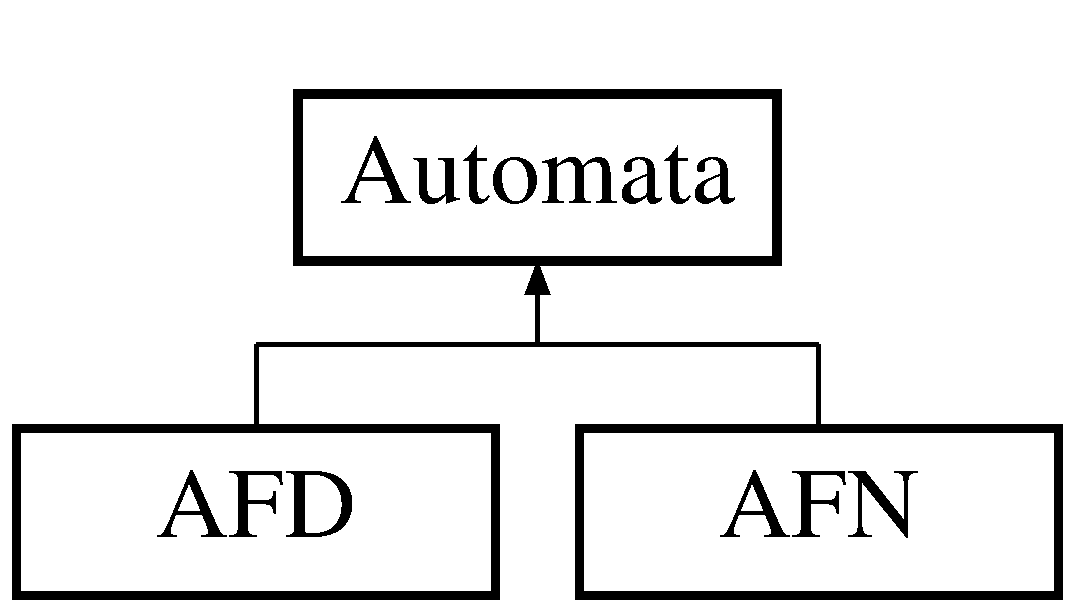
\includegraphics[height=2.000000cm]{class_automata}
\end{center}
\end{figure}
\subsection*{Public Member Functions}
\begin{DoxyCompactItemize}
\item 
\hyperlink{class_automata_ae13e4a7c4d7f0291c80b252a2510ebff}{Automata} ()
\item 
\mbox{\Hypertarget{class_automata_aa47afd5e2da0635037e6bd8c016d1f2c}\label{class_automata_aa47afd5e2da0635037e6bd8c016d1f2c}} 
{\bfseries Automata} (std\+::string archivo, std\+::string tipo)
\item 
\mbox{\Hypertarget{class_automata_a9842cc66caee1a9a3ded188753bdc863}\label{class_automata_a9842cc66caee1a9a3ded188753bdc863}} 
{\bfseries Automata} (std\+::vector$<$ \hyperlink{class_estado}{Estado} $\ast$$>$ estados, std\+::vector$<$ char $>$ alfabeto, \hyperlink{class_estado}{Estado} $\ast$estado\+Inicial, std\+::vector$<$ \hyperlink{class_transicion}{Transicion} $\ast$$>$ tabla\+De\+Transiciones)
\item 
\mbox{\Hypertarget{class_automata_aaac8c053963a3aa29ccb2553c8c5a212}\label{class_automata_aaac8c053963a3aa29ccb2553c8c5a212}} 
{\bfseries Automata} (std\+::vector$<$ \hyperlink{class_estado}{Estado} $\ast$$>$ estados, std\+::vector$<$ char $>$ alfabeto, \hyperlink{class_estado}{Estado} $\ast$estado\+Inicial, \hyperlink{class_estado}{Estado} $\ast$estado\+Final, std\+::vector$<$ \hyperlink{class_transicion}{Transicion} $\ast$$>$ tabla\+De\+Transiciones)
\item 
std\+::vector$<$ \hyperlink{class_estado}{Estado} $\ast$ $>$ \hyperlink{class_automata_a9c728bd19771264ac35e95fd8b97069a}{obtener\+Estados} ()
\item 
std\+::vector$<$ \hyperlink{class_transicion}{Transicion} $\ast$ $>$ \hyperlink{class_automata_ae2b571c39f955aafb293ea9605a4a1bb}{obtener\+Tabla\+De\+Transiciones} ()
\item 
std\+::vector$<$ char $>$ \hyperlink{class_automata_af82a91d0826881327ee4b05723961c2f}{obtener\+Alfabeto} ()
\item 
\hyperlink{class_estado}{Estado} $\ast$ \hyperlink{class_automata_a00cdbcd4da13f79ce9b80935ca54eee7}{obtener\+Estado\+Inicial} ()
\item 
\hyperlink{class_estado}{Estado} $\ast$ \hyperlink{class_automata_a0aa43eed6361c006212719a97ffd920d}{obtener\+Estado\+Final} ()
\item 
std\+::vector$<$ \hyperlink{class_estado}{Estado} $\ast$ $>$ \hyperlink{class_automata_a57e9a913a7264f19b14401f01110df24}{obtener\+Estados\+Finales} ()
\item 
void \hyperlink{class_automata_ac95575b672e736c6f1bcc75f4cacf15d}{to\+String} (std\+::string tipo)
\end{DoxyCompactItemize}
\subsection*{Public Attributes}
\begin{DoxyCompactItemize}
\item 
\mbox{\Hypertarget{class_automata_a1fd6b03f285f603487068124245cdf92}\label{class_automata_a1fd6b03f285f603487068124245cdf92}} 
std\+::vector$<$ \hyperlink{class_estado}{Estado} $\ast$ $>$ {\bfseries automata\+\_\+estados}
\item 
\mbox{\Hypertarget{class_automata_af8729647a199dccc401cae627ce6c45c}\label{class_automata_af8729647a199dccc401cae627ce6c45c}} 
std\+::vector$<$ char $>$ {\bfseries automata\+\_\+alfabeto}
\item 
\mbox{\Hypertarget{class_automata_a4943b6542bba80e61b748db0bf769313}\label{class_automata_a4943b6542bba80e61b748db0bf769313}} 
\hyperlink{class_estado}{Estado} $\ast$ {\bfseries automata\+\_\+estado\+Inicial}
\item 
\mbox{\Hypertarget{class_automata_ae504d2338c97b59afbbe24a5d3119c73}\label{class_automata_ae504d2338c97b59afbbe24a5d3119c73}} 
\hyperlink{class_estado}{Estado} $\ast$ {\bfseries automata\+\_\+estado\+Final}
\item 
\mbox{\Hypertarget{class_automata_a1c95a0ef7a011e66cb6ee216b0bbbca6}\label{class_automata_a1c95a0ef7a011e66cb6ee216b0bbbca6}} 
std\+::vector$<$ \hyperlink{class_transicion}{Transicion} $\ast$ $>$ {\bfseries automata\+\_\+tabla\+De\+Transiciones}
\end{DoxyCompactItemize}


\subsection{Constructor \& Destructor Documentation}
\mbox{\Hypertarget{class_automata_ae13e4a7c4d7f0291c80b252a2510ebff}\label{class_automata_ae13e4a7c4d7f0291c80b252a2510ebff}} 
\index{Automata@{Automata}!Automata@{Automata}}
\index{Automata@{Automata}!Automata@{Automata}}
\subsubsection{\texorpdfstring{Automata()}{Automata()}}
{\footnotesize\ttfamily Automata\+::\+Automata (\begin{DoxyParamCaption}{ }\end{DoxyParamCaption})}

Constructor 

\subsection{Member Function Documentation}
\mbox{\Hypertarget{class_automata_af82a91d0826881327ee4b05723961c2f}\label{class_automata_af82a91d0826881327ee4b05723961c2f}} 
\index{Automata@{Automata}!obtener\+Alfabeto@{obtener\+Alfabeto}}
\index{obtener\+Alfabeto@{obtener\+Alfabeto}!Automata@{Automata}}
\subsubsection{\texorpdfstring{obtener\+Alfabeto()}{obtenerAlfabeto()}}
{\footnotesize\ttfamily vector$<$ char $>$ Automata\+::obtener\+Alfabeto (\begin{DoxyParamCaption}{ }\end{DoxyParamCaption})}

Esta funcion obtiene alfabeto del automata \mbox{\Hypertarget{class_automata_a0aa43eed6361c006212719a97ffd920d}\label{class_automata_a0aa43eed6361c006212719a97ffd920d}} 
\index{Automata@{Automata}!obtener\+Estado\+Final@{obtener\+Estado\+Final}}
\index{obtener\+Estado\+Final@{obtener\+Estado\+Final}!Automata@{Automata}}
\subsubsection{\texorpdfstring{obtener\+Estado\+Final()}{obtenerEstadoFinal()}}
{\footnotesize\ttfamily \hyperlink{class_estado}{Estado} $\ast$ Automata\+::obtener\+Estado\+Final (\begin{DoxyParamCaption}{ }\end{DoxyParamCaption})}

Esta funcion obtiene el estado final del automata \mbox{\Hypertarget{class_automata_a00cdbcd4da13f79ce9b80935ca54eee7}\label{class_automata_a00cdbcd4da13f79ce9b80935ca54eee7}} 
\index{Automata@{Automata}!obtener\+Estado\+Inicial@{obtener\+Estado\+Inicial}}
\index{obtener\+Estado\+Inicial@{obtener\+Estado\+Inicial}!Automata@{Automata}}
\subsubsection{\texorpdfstring{obtener\+Estado\+Inicial()}{obtenerEstadoInicial()}}
{\footnotesize\ttfamily \hyperlink{class_estado}{Estado} $\ast$ Automata\+::obtener\+Estado\+Inicial (\begin{DoxyParamCaption}{ }\end{DoxyParamCaption})}

Esta funcion obtiene el estado inicial del automata \mbox{\Hypertarget{class_automata_a9c728bd19771264ac35e95fd8b97069a}\label{class_automata_a9c728bd19771264ac35e95fd8b97069a}} 
\index{Automata@{Automata}!obtener\+Estados@{obtener\+Estados}}
\index{obtener\+Estados@{obtener\+Estados}!Automata@{Automata}}
\subsubsection{\texorpdfstring{obtener\+Estados()}{obtenerEstados()}}
{\footnotesize\ttfamily vector$<$ \hyperlink{class_estado}{Estado} $\ast$ $>$ Automata\+::obtener\+Estados (\begin{DoxyParamCaption}{ }\end{DoxyParamCaption})}

Esta funcion obtiene el vector de estados del automata \mbox{\Hypertarget{class_automata_a57e9a913a7264f19b14401f01110df24}\label{class_automata_a57e9a913a7264f19b14401f01110df24}} 
\index{Automata@{Automata}!obtener\+Estados\+Finales@{obtener\+Estados\+Finales}}
\index{obtener\+Estados\+Finales@{obtener\+Estados\+Finales}!Automata@{Automata}}
\subsubsection{\texorpdfstring{obtener\+Estados\+Finales()}{obtenerEstadosFinales()}}
{\footnotesize\ttfamily vector$<$ \hyperlink{class_estado}{Estado} $\ast$ $>$ Automata\+::obtener\+Estados\+Finales (\begin{DoxyParamCaption}{ }\end{DoxyParamCaption})}

Esta funcion obtiene el conjunto de estados finales del automata Regresa\+:
\begin{DoxyItemize}
\item vector$<$\+Estado$\ast$$>$ finales \+:\+: El conjunto de estados finales. 
\end{DoxyItemize}\mbox{\Hypertarget{class_automata_ae2b571c39f955aafb293ea9605a4a1bb}\label{class_automata_ae2b571c39f955aafb293ea9605a4a1bb}} 
\index{Automata@{Automata}!obtener\+Tabla\+De\+Transiciones@{obtener\+Tabla\+De\+Transiciones}}
\index{obtener\+Tabla\+De\+Transiciones@{obtener\+Tabla\+De\+Transiciones}!Automata@{Automata}}
\subsubsection{\texorpdfstring{obtener\+Tabla\+De\+Transiciones()}{obtenerTablaDeTransiciones()}}
{\footnotesize\ttfamily vector$<$ \hyperlink{class_transicion}{Transicion} $\ast$ $>$ Automata\+::obtener\+Tabla\+De\+Transiciones (\begin{DoxyParamCaption}{ }\end{DoxyParamCaption})}

Esta funcion obtiene la tablade transiciones del automata \mbox{\Hypertarget{class_automata_ac95575b672e736c6f1bcc75f4cacf15d}\label{class_automata_ac95575b672e736c6f1bcc75f4cacf15d}} 
\index{Automata@{Automata}!to\+String@{to\+String}}
\index{to\+String@{to\+String}!Automata@{Automata}}
\subsubsection{\texorpdfstring{to\+String()}{toString()}}
{\footnotesize\ttfamily void Automata\+::to\+String (\begin{DoxyParamCaption}\item[{std\+::string}]{tipo }\end{DoxyParamCaption})}

Metodo to\+String de la clase \hyperlink{class_automata}{Automata}, imprime la informacion del automata. 

The documentation for this class was generated from the following files\+:\begin{DoxyCompactItemize}
\item 
Automata.\+hpp\item 
Automata.\+cpp\end{DoxyCompactItemize}

\hypertarget{class_estado}{}\section{Estado Class Reference}
\label{class_estado}\index{Estado@{Estado}}
\subsection*{Public Member Functions}
\begin{DoxyCompactItemize}
\item 
\hyperlink{class_estado_a916fc52f64ed19c1ea86acbcc9a83b4f}{Estado} (int num\+De\+Estado, bool tipo)
\end{DoxyCompactItemize}
\subsection*{Public Attributes}
\begin{DoxyCompactItemize}
\item 
\mbox{\Hypertarget{class_estado_af32184e41b6771d7855b7e4a7c0b1758}\label{class_estado_af32184e41b6771d7855b7e4a7c0b1758}} 
int {\bfseries numero\+De\+Estado}
\item 
\mbox{\Hypertarget{class_estado_aae3487981a5e4395fc6156ef5fc35376}\label{class_estado_aae3487981a5e4395fc6156ef5fc35376}} 
bool {\bfseries es\+Final}
\end{DoxyCompactItemize}


\subsection{Constructor \& Destructor Documentation}
\mbox{\Hypertarget{class_estado_a916fc52f64ed19c1ea86acbcc9a83b4f}\label{class_estado_a916fc52f64ed19c1ea86acbcc9a83b4f}} 
\index{Estado@{Estado}!Estado@{Estado}}
\index{Estado@{Estado}!Estado@{Estado}}
\subsubsection{\texorpdfstring{Estado()}{Estado()}}
{\footnotesize\ttfamily Estado\+::\+Estado (\begin{DoxyParamCaption}\item[{int}]{num\+De\+Estado,  }\item[{bool}]{tipo }\end{DoxyParamCaption})}

Constructor 

The documentation for this class was generated from the following files\+:\begin{DoxyCompactItemize}
\item 
Estado.\+hpp\item 
Estado.\+cpp\end{DoxyCompactItemize}

\hypertarget{class_pruebas}{}\section{Pruebas Class Reference}
\label{class_pruebas}\index{Pruebas@{Pruebas}}
Inheritance diagram for Pruebas\+:\begin{figure}[H]
\begin{center}
\leavevmode
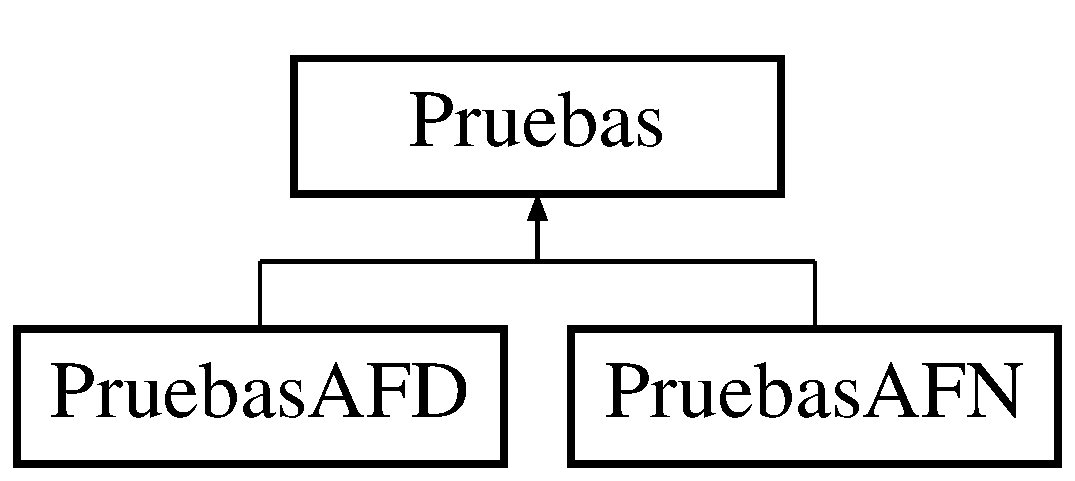
\includegraphics[height=2.000000cm]{class_pruebas}
\end{center}
\end{figure}
\subsection*{Public Member Functions}
\begin{DoxyCompactItemize}
\item 
\hyperlink{class_pruebas_af78514bc056a28b5477af6b75216364e}{Pruebas} ()
\item 
bool \hyperlink{class_pruebas_ab1eda5c03c5298ba35c48845ff6544eb}{buscar\+Simbolo} (std\+::vector$<$ char $>$ alfabeto, char simbolo)
\item 
std\+::vector$<$ char $>$ \hyperlink{class_pruebas_a4f7adc9be1f1f9ec96d6a713c728f4cc}{definir\+Alfabeto} (int numero\+De\+Simbolos)
\item 
std\+::vector$<$ \hyperlink{class_estado}{Estado} $\ast$ $>$ \hyperlink{class_pruebas_a7d80b5a28534edbf0f92f56e8e423f3e}{agregar\+Estados} (int numero\+De\+Estados)
\end{DoxyCompactItemize}


\subsection{Constructor \& Destructor Documentation}
\mbox{\Hypertarget{class_pruebas_af78514bc056a28b5477af6b75216364e}\label{class_pruebas_af78514bc056a28b5477af6b75216364e}} 
\index{Pruebas@{Pruebas}!Pruebas@{Pruebas}}
\index{Pruebas@{Pruebas}!Pruebas@{Pruebas}}
\subsubsection{\texorpdfstring{Pruebas()}{Pruebas()}}
{\footnotesize\ttfamily Pruebas\+::\+Pruebas (\begin{DoxyParamCaption}{ }\end{DoxyParamCaption})}

Constructor 

\subsection{Member Function Documentation}
\mbox{\Hypertarget{class_pruebas_a7d80b5a28534edbf0f92f56e8e423f3e}\label{class_pruebas_a7d80b5a28534edbf0f92f56e8e423f3e}} 
\index{Pruebas@{Pruebas}!agregar\+Estados@{agregar\+Estados}}
\index{agregar\+Estados@{agregar\+Estados}!Pruebas@{Pruebas}}
\subsubsection{\texorpdfstring{agregar\+Estados()}{agregarEstados()}}
{\footnotesize\ttfamily vector$<$ \hyperlink{class_estado}{Estado} $\ast$ $>$ Pruebas\+::agregar\+Estados (\begin{DoxyParamCaption}\item[{int}]{numero\+De\+Estados }\end{DoxyParamCaption})}

Esta funcion permite agregar estados al automata. Recibe\+:
\begin{DoxyItemize}
\item int numero\+De\+Estados \+:\+: la cantidad de estados a agregar. Regresa\+:
\item vector$<$\+Estado$\ast$$>$ estados \+:\+: El vector de estados 
\end{DoxyItemize}\mbox{\Hypertarget{class_pruebas_ab1eda5c03c5298ba35c48845ff6544eb}\label{class_pruebas_ab1eda5c03c5298ba35c48845ff6544eb}} 
\index{Pruebas@{Pruebas}!buscar\+Simbolo@{buscar\+Simbolo}}
\index{buscar\+Simbolo@{buscar\+Simbolo}!Pruebas@{Pruebas}}
\subsubsection{\texorpdfstring{buscar\+Simbolo()}{buscarSimbolo()}}
{\footnotesize\ttfamily bool Pruebas\+::buscar\+Simbolo (\begin{DoxyParamCaption}\item[{std\+::vector$<$ char $>$}]{alfabeto,  }\item[{char}]{simbolo }\end{DoxyParamCaption})}

Esta funcion determina si un simbolo pertenece al alfabeto del automata. Recibe\+:
\begin{DoxyItemize}
\item vector$<$char$>$ alfabeto \+:\+: El alfabeto del automata
\item char simbolo \+:\+: El simbolo a buscar en el automata Regresa\+:
\item true \+:\+: si se encontro el simbolo
\item false \+:\+: si no se encontro el simbolo 
\end{DoxyItemize}\mbox{\Hypertarget{class_pruebas_a4f7adc9be1f1f9ec96d6a713c728f4cc}\label{class_pruebas_a4f7adc9be1f1f9ec96d6a713c728f4cc}} 
\index{Pruebas@{Pruebas}!definir\+Alfabeto@{definir\+Alfabeto}}
\index{definir\+Alfabeto@{definir\+Alfabeto}!Pruebas@{Pruebas}}
\subsubsection{\texorpdfstring{definir\+Alfabeto()}{definirAlfabeto()}}
{\footnotesize\ttfamily vector$<$ char $>$ Pruebas\+::definir\+Alfabeto (\begin{DoxyParamCaption}\item[{int}]{numero\+De\+Simbolos }\end{DoxyParamCaption})}

Esta funcion define el alfabeto del automata. Recibe\+:
\begin{DoxyItemize}
\item int numero\+De\+Simbolos \+:\+: El numero de simbolos del alfabeto Regresa\+:
\item vector$<$char$>$ alfabeto\+Aux \+:\+: El alfabeto generado 
\end{DoxyItemize}

The documentation for this class was generated from the following files\+:\begin{DoxyCompactItemize}
\item 
Pruebas.\+hpp\item 
Pruebas.\+cpp\end{DoxyCompactItemize}

\hypertarget{class_pruebas_a_f_d}{}\section{Pruebas\+A\+FD Class Reference}
\label{class_pruebas_a_f_d}\index{Pruebas\+A\+FD@{Pruebas\+A\+FD}}
Inheritance diagram for Pruebas\+A\+FD\+:\begin{figure}[H]
\begin{center}
\leavevmode
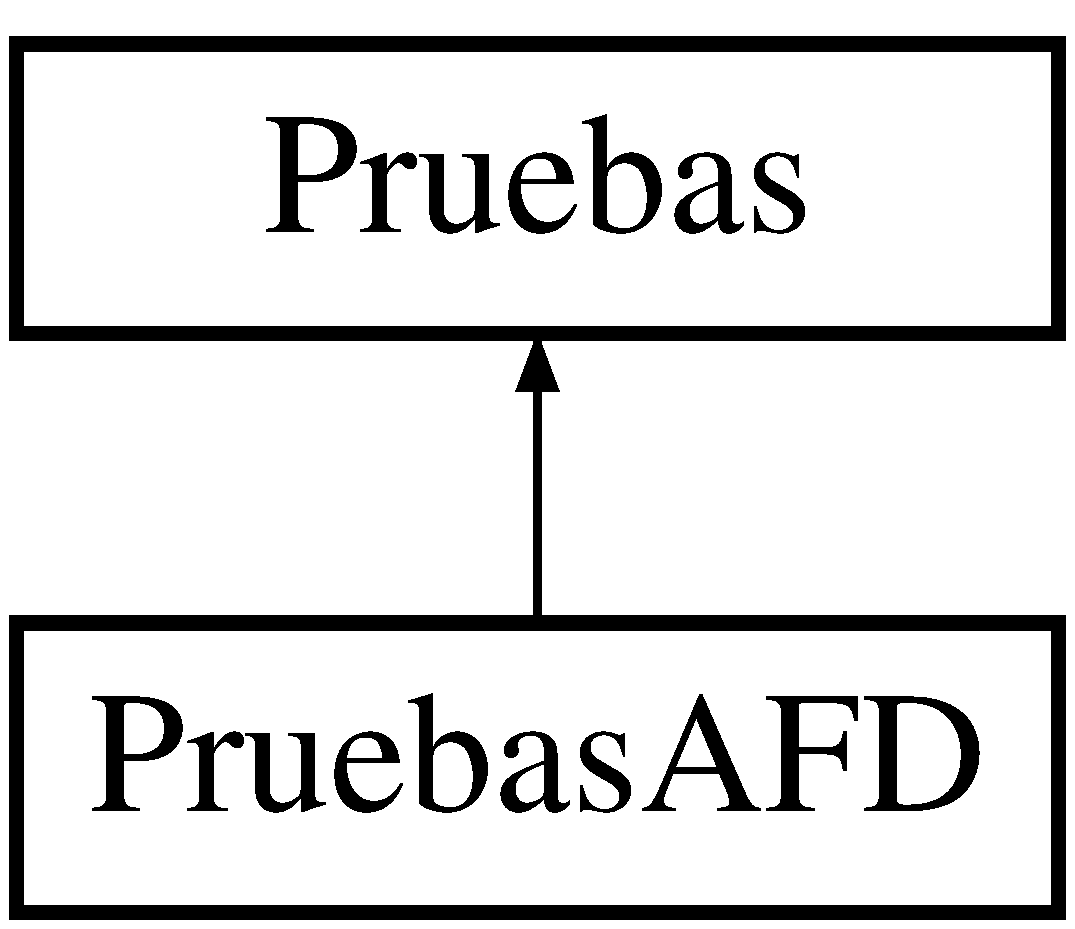
\includegraphics[height=2.000000cm]{class_pruebas_a_f_d}
\end{center}
\end{figure}
\subsection*{Public Member Functions}
\begin{DoxyCompactItemize}
\item 
std\+::vector$<$ \hyperlink{class_transicion}{Transicion} $\ast$ $>$ \hyperlink{class_pruebas_a_f_d_a991ac328ebeae3ca84958887cbf4e41d}{definir\+Transiciones\+A\+FD} (int numero\+De\+Transiciones, std\+::vector$<$ char $>$ alfabeto)
\item 
bool \hyperlink{class_pruebas_a_f_d_ae8c9889569bc90bc8f55c3b09c4570eb}{iniciar\+Prueba\+A\+FD} (\hyperlink{class_a_f_d}{A\+FD} automata\+De\+Prueba)
\item 
void \hyperlink{class_pruebas_a_f_d_ab377ec9490bd437af165410a3ff10fd4}{probar\+Cadenas\+A\+FD} (\hyperlink{class_a_f_d}{A\+FD} automata\+De\+Prueba)
\item 
void \hyperlink{class_pruebas_a_f_d_acecc332248164ed9dc6b37029e0c0f33}{crear\+A\+FD} ()
\end{DoxyCompactItemize}


\subsection{Member Function Documentation}
\mbox{\Hypertarget{class_pruebas_a_f_d_acecc332248164ed9dc6b37029e0c0f33}\label{class_pruebas_a_f_d_acecc332248164ed9dc6b37029e0c0f33}} 
\index{Pruebas\+A\+FD@{Pruebas\+A\+FD}!crear\+A\+FD@{crear\+A\+FD}}
\index{crear\+A\+FD@{crear\+A\+FD}!Pruebas\+A\+FD@{Pruebas\+A\+FD}}
\subsubsection{\texorpdfstring{crear\+A\+F\+D()}{crearAFD()}}
{\footnotesize\ttfamily void Pruebas\+A\+F\+D\+::crear\+A\+FD (\begin{DoxyParamCaption}{ }\end{DoxyParamCaption})}

Esta funcion permite crear un \hyperlink{class_a_f_d}{A\+FD} a partir de un archivo o ingresando informacion desde consola. \mbox{\Hypertarget{class_pruebas_a_f_d_a991ac328ebeae3ca84958887cbf4e41d}\label{class_pruebas_a_f_d_a991ac328ebeae3ca84958887cbf4e41d}} 
\index{Pruebas\+A\+FD@{Pruebas\+A\+FD}!definir\+Transiciones\+A\+FD@{definir\+Transiciones\+A\+FD}}
\index{definir\+Transiciones\+A\+FD@{definir\+Transiciones\+A\+FD}!Pruebas\+A\+FD@{Pruebas\+A\+FD}}
\subsubsection{\texorpdfstring{definir\+Transiciones\+A\+F\+D()}{definirTransicionesAFD()}}
{\footnotesize\ttfamily vector$<$ \hyperlink{class_transicion}{Transicion} $\ast$ $>$ Pruebas\+A\+F\+D\+::definir\+Transiciones\+A\+FD (\begin{DoxyParamCaption}\item[{int}]{numero\+De\+Transiciones,  }\item[{std\+::vector$<$ char $>$}]{alfabeto }\end{DoxyParamCaption})}

Esta funcion permite definir las transiciones del automata \hyperlink{class_a_f_d}{A\+FD}. Recibe\+:
\begin{DoxyItemize}
\item int numero\+De\+Transiciones \+:\+: El numero de transiciones a definir
\item vector$<$char$>$ alfabeto \+:\+: El alfabeto del automata Regresa\+:
\item vector$<$\+Transicion$\ast$$>$ transiciones \+:\+: La tabla de transiciones del \hyperlink{class_a_f_d}{A\+FD} 
\end{DoxyItemize}\mbox{\Hypertarget{class_pruebas_a_f_d_ae8c9889569bc90bc8f55c3b09c4570eb}\label{class_pruebas_a_f_d_ae8c9889569bc90bc8f55c3b09c4570eb}} 
\index{Pruebas\+A\+FD@{Pruebas\+A\+FD}!iniciar\+Prueba\+A\+FD@{iniciar\+Prueba\+A\+FD}}
\index{iniciar\+Prueba\+A\+FD@{iniciar\+Prueba\+A\+FD}!Pruebas\+A\+FD@{Pruebas\+A\+FD}}
\subsubsection{\texorpdfstring{iniciar\+Prueba\+A\+F\+D()}{iniciarPruebaAFD()}}
{\footnotesize\ttfamily bool Pruebas\+A\+F\+D\+::iniciar\+Prueba\+A\+FD (\begin{DoxyParamCaption}\item[{\hyperlink{class_a_f_d}{A\+FD}}]{automata\+De\+Prueba }\end{DoxyParamCaption})}

Esta funcion ejecuta pruebas con cadenas en un automata \hyperlink{class_a_f_d}{A\+FD}. Recibe\+: -\/\+A\+FD automata\+De\+Prueba \+:\+: \hyperlink{class_automata}{Automata} para la prueba. Regresa\+: -\/true \+:\+: si la cadena fue reconocida por el \hyperlink{class_a_f_d}{A\+FD} -\/false \+:\+: si la cadena no fue reconocida por el \hyperlink{class_a_f_d}{A\+FD} \mbox{\Hypertarget{class_pruebas_a_f_d_ab377ec9490bd437af165410a3ff10fd4}\label{class_pruebas_a_f_d_ab377ec9490bd437af165410a3ff10fd4}} 
\index{Pruebas\+A\+FD@{Pruebas\+A\+FD}!probar\+Cadenas\+A\+FD@{probar\+Cadenas\+A\+FD}}
\index{probar\+Cadenas\+A\+FD@{probar\+Cadenas\+A\+FD}!Pruebas\+A\+FD@{Pruebas\+A\+FD}}
\subsubsection{\texorpdfstring{probar\+Cadenas\+A\+F\+D()}{probarCadenasAFD()}}
{\footnotesize\ttfamily void Pruebas\+A\+F\+D\+::probar\+Cadenas\+A\+FD (\begin{DoxyParamCaption}\item[{\hyperlink{class_a_f_d}{A\+FD}}]{automata\+De\+Prueba }\end{DoxyParamCaption})}

Esta funcion prueba una cadena en un \hyperlink{class_a_f_d}{A\+FD} con base a su funcion de transicion. Recibe\+:
\begin{DoxyItemize}
\item \hyperlink{class_a_f_d}{A\+FD} automata\+De\+Prueba \+:\+: El automata \hyperlink{class_a_f_d}{A\+FD} a probar 
\end{DoxyItemize}

The documentation for this class was generated from the following files\+:\begin{DoxyCompactItemize}
\item 
Pruebas\+A\+F\+D.\+hpp\item 
Pruebas\+A\+F\+D.\+cpp\end{DoxyCompactItemize}

\hypertarget{class_pruebas_a_f_n}{}\section{Pruebas\+A\+FN Class Reference}
\label{class_pruebas_a_f_n}\index{Pruebas\+A\+FN@{Pruebas\+A\+FN}}
Inheritance diagram for Pruebas\+A\+FN\+:\begin{figure}[H]
\begin{center}
\leavevmode
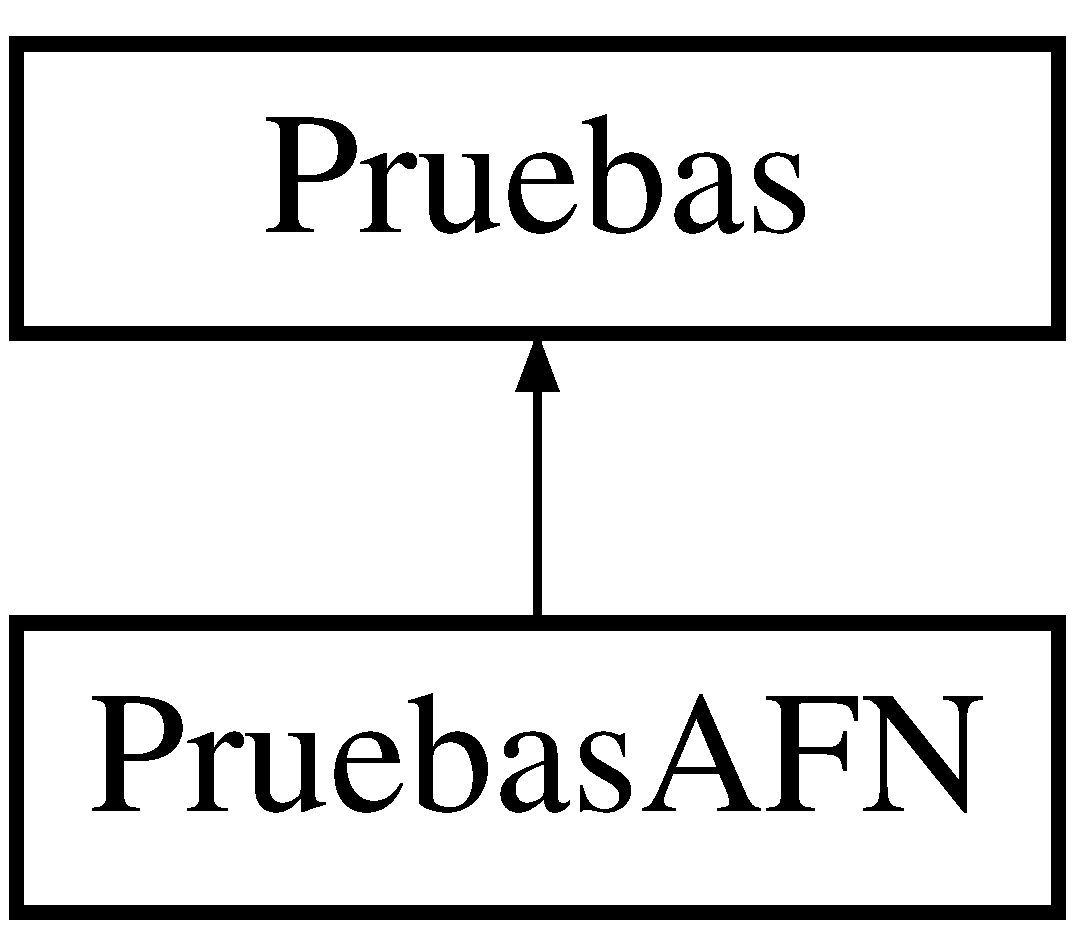
\includegraphics[height=2.000000cm]{class_pruebas_a_f_n}
\end{center}
\end{figure}
\subsection*{Public Member Functions}
\begin{DoxyCompactItemize}
\item 
std\+::vector$<$ \hyperlink{class_transicion}{Transicion} $\ast$ $>$ \hyperlink{class_pruebas_a_f_n_ab895e1c3ac049325060b898084a22a61}{definir\+Transiciones\+A\+FN} (int numero\+De\+Transiciones, std\+::vector$<$ char $>$ alfabeto)
\item 
bool \hyperlink{class_pruebas_a_f_n_a8d6784ce185b05b5e454274674b0a63f}{iniciar\+Prueba\+A\+FN} (\hyperlink{class_a_f_n}{A\+FN} automata\+De\+Prueba)
\item 
bool \hyperlink{class_pruebas_a_f_n_aae54c0ea1b237f04b5b3f8625a1b58d2}{no\+Es\+Especial} (char a)
\item 
void \hyperlink{class_pruebas_a_f_n_a9349654408b4c931fd854f8cd304d324}{probar\+Cadenas\+A\+FN} (\hyperlink{class_a_f_n}{A\+FN} automata\+De\+Prueba)
\item 
void \hyperlink{class_pruebas_a_f_n_a1df5917c3e8b3f2dc1f83744ad30ffdb}{crear\+A\+FN} ()
\item 
\hyperlink{class_a_f_n}{A\+FN} \hyperlink{class_pruebas_a_f_n_a6fe30bfd1b6d13a1ac3a2ad6a6b70750}{convertir\+E\+Ra\+A\+FN} (std\+::string expresion\+Regular)
\end{DoxyCompactItemize}


\subsection{Member Function Documentation}
\mbox{\Hypertarget{class_pruebas_a_f_n_a6fe30bfd1b6d13a1ac3a2ad6a6b70750}\label{class_pruebas_a_f_n_a6fe30bfd1b6d13a1ac3a2ad6a6b70750}} 
\index{Pruebas\+A\+FN@{Pruebas\+A\+FN}!convertir\+E\+Ra\+A\+FN@{convertir\+E\+Ra\+A\+FN}}
\index{convertir\+E\+Ra\+A\+FN@{convertir\+E\+Ra\+A\+FN}!Pruebas\+A\+FN@{Pruebas\+A\+FN}}
\subsubsection{\texorpdfstring{convertir\+E\+Ra\+A\+F\+N()}{convertirERaAFN()}}
{\footnotesize\ttfamily \hyperlink{class_a_f_n}{A\+FN} Pruebas\+A\+F\+N\+::convertir\+E\+Ra\+A\+FN (\begin{DoxyParamCaption}\item[{std\+::string}]{expresion\+Regular }\end{DoxyParamCaption})}

Esta funcion permite convertir una expresion regular en un \hyperlink{class_a_f_n}{A\+FN} usando las construcciones de Thompson. Recibe\+:
\begin{DoxyItemize}
\item string expresion\+Regular \+:\+: cadena que representa a la expresion regular Regresa\+: \hyperlink{class_a_f_n}{A\+FN} afn \+:\+: El automata finito no determinista que reconoce el lenguaje generado por la expresion regular, hecho mediante las construcciones de Thompson. 
\end{DoxyItemize}\mbox{\Hypertarget{class_pruebas_a_f_n_a1df5917c3e8b3f2dc1f83744ad30ffdb}\label{class_pruebas_a_f_n_a1df5917c3e8b3f2dc1f83744ad30ffdb}} 
\index{Pruebas\+A\+FN@{Pruebas\+A\+FN}!crear\+A\+FN@{crear\+A\+FN}}
\index{crear\+A\+FN@{crear\+A\+FN}!Pruebas\+A\+FN@{Pruebas\+A\+FN}}
\subsubsection{\texorpdfstring{crear\+A\+F\+N()}{crearAFN()}}
{\footnotesize\ttfamily void Pruebas\+A\+F\+N\+::crear\+A\+FN (\begin{DoxyParamCaption}{ }\end{DoxyParamCaption})}

Esta funcion permite crear un \hyperlink{class_a_f_n}{A\+FN} a partir de un archivo o ingresando informacion desde consola. \mbox{\Hypertarget{class_pruebas_a_f_n_ab895e1c3ac049325060b898084a22a61}\label{class_pruebas_a_f_n_ab895e1c3ac049325060b898084a22a61}} 
\index{Pruebas\+A\+FN@{Pruebas\+A\+FN}!definir\+Transiciones\+A\+FN@{definir\+Transiciones\+A\+FN}}
\index{definir\+Transiciones\+A\+FN@{definir\+Transiciones\+A\+FN}!Pruebas\+A\+FN@{Pruebas\+A\+FN}}
\subsubsection{\texorpdfstring{definir\+Transiciones\+A\+F\+N()}{definirTransicionesAFN()}}
{\footnotesize\ttfamily vector$<$ \hyperlink{class_transicion}{Transicion} $\ast$ $>$ Pruebas\+A\+F\+N\+::definir\+Transiciones\+A\+FN (\begin{DoxyParamCaption}\item[{int}]{numero\+De\+Transiciones,  }\item[{std\+::vector$<$ char $>$}]{alfabeto }\end{DoxyParamCaption})}

Esta funcion permite definir las transiciones del automata \hyperlink{class_a_f_n}{A\+FN}. Recibe\+:
\begin{DoxyItemize}
\item int numero\+De\+Transiciones \+:\+: El numero de transiciones a definir
\item vector$<$char$>$ alfabeto \+:\+: El alfabeto del automata Regresa\+:
\item vector$<$\+Transicion$\ast$$>$ transiciones \+:\+: La tabla de transiciones del \hyperlink{class_a_f_n}{A\+FN} 
\end{DoxyItemize}\mbox{\Hypertarget{class_pruebas_a_f_n_a8d6784ce185b05b5e454274674b0a63f}\label{class_pruebas_a_f_n_a8d6784ce185b05b5e454274674b0a63f}} 
\index{Pruebas\+A\+FN@{Pruebas\+A\+FN}!iniciar\+Prueba\+A\+FN@{iniciar\+Prueba\+A\+FN}}
\index{iniciar\+Prueba\+A\+FN@{iniciar\+Prueba\+A\+FN}!Pruebas\+A\+FN@{Pruebas\+A\+FN}}
\subsubsection{\texorpdfstring{iniciar\+Prueba\+A\+F\+N()}{iniciarPruebaAFN()}}
{\footnotesize\ttfamily bool Pruebas\+A\+F\+N\+::iniciar\+Prueba\+A\+FN (\begin{DoxyParamCaption}\item[{\hyperlink{class_a_f_n}{A\+FN}}]{automata\+De\+Prueba }\end{DoxyParamCaption})}

Esta funcion ejecuta pruebas con cadenas en un automata \hyperlink{class_a_f_n}{A\+FN}. Recibe\+: -\/\+A\+FN automata\+De\+Prueba \+:\+: \hyperlink{class_automata}{Automata} para la prueba. Regresa\+: -\/true \+:\+: si la cadena fue reconocida por el \hyperlink{class_a_f_n}{A\+FN} -\/false \+:\+: si la cadena no fue reconocida por el \hyperlink{class_a_f_n}{A\+FN} \mbox{\Hypertarget{class_pruebas_a_f_n_aae54c0ea1b237f04b5b3f8625a1b58d2}\label{class_pruebas_a_f_n_aae54c0ea1b237f04b5b3f8625a1b58d2}} 
\index{Pruebas\+A\+FN@{Pruebas\+A\+FN}!no\+Es\+Especial@{no\+Es\+Especial}}
\index{no\+Es\+Especial@{no\+Es\+Especial}!Pruebas\+A\+FN@{Pruebas\+A\+FN}}
\subsubsection{\texorpdfstring{no\+Es\+Especial()}{noEsEspecial()}}
{\footnotesize\ttfamily bool Pruebas\+A\+F\+N\+::no\+Es\+Especial (\begin{DoxyParamCaption}\item[{char}]{a }\end{DoxyParamCaption})}

Esta funcion comprueba que un caracter no sea el caracter nulo o alguno de los caracteres especiales utilizados para definir expresiones regulares. Recibe\+:
\begin{DoxyItemize}
\item char a \+:\+: caracter a evaluar Regresa\+:
\item true \+:\+: si el caracter no pertenece a un operador de ER o el caracter nulo
\item false \+:\+: si es un operador de ER o es el caracter nulo 
\end{DoxyItemize}\mbox{\Hypertarget{class_pruebas_a_f_n_a9349654408b4c931fd854f8cd304d324}\label{class_pruebas_a_f_n_a9349654408b4c931fd854f8cd304d324}} 
\index{Pruebas\+A\+FN@{Pruebas\+A\+FN}!probar\+Cadenas\+A\+FN@{probar\+Cadenas\+A\+FN}}
\index{probar\+Cadenas\+A\+FN@{probar\+Cadenas\+A\+FN}!Pruebas\+A\+FN@{Pruebas\+A\+FN}}
\subsubsection{\texorpdfstring{probar\+Cadenas\+A\+F\+N()}{probarCadenasAFN()}}
{\footnotesize\ttfamily void Pruebas\+A\+F\+N\+::probar\+Cadenas\+A\+FN (\begin{DoxyParamCaption}\item[{\hyperlink{class_a_f_n}{A\+FN}}]{automata\+De\+Prueba }\end{DoxyParamCaption})}

Esta funcion prueba una cadena en un \hyperlink{class_a_f_n}{A\+FN} con base a su funcion de transicion. Recibe\+:
\begin{DoxyItemize}
\item \hyperlink{class_a_f_n}{A\+FN} automata\+De\+Prueba \+:\+: El automata \hyperlink{class_a_f_n}{A\+FN} a probar 
\end{DoxyItemize}

The documentation for this class was generated from the following files\+:\begin{DoxyCompactItemize}
\item 
Pruebas\+A\+F\+N.\+hpp\item 
Pruebas\+A\+F\+N.\+cpp\end{DoxyCompactItemize}

\hypertarget{class_subconjunto}{}\section{Subconjunto Class Reference}
\label{class_subconjunto}\index{Subconjunto@{Subconjunto}}
\subsection*{Public Member Functions}
\begin{DoxyCompactItemize}
\item 
void \hyperlink{class_subconjunto_aa8b327da2cfd9c8fb1d0b42edc737322}{iniciar\+Algoritmo} ()
\item 
void \hyperlink{class_subconjunto_a41444a0c990781527ae37a2e4374a516}{generar\+Tabla\+De\+Preprocesamiento} (\hyperlink{class_a_f_n}{A\+FN} afn)
\item 
void \hyperlink{class_subconjunto_a3b5add3ea0f5d4b11b226ffe18cbcbb0}{procesar\+Estado\+Inicial} (\hyperlink{class_a_f_n}{A\+FN} afn)
\item 
\mbox{\Hypertarget{class_subconjunto_a1d606dfc6d781751d5d8bae5a9c7c034}\label{class_subconjunto_a1d606dfc6d781751d5d8bae5a9c7c034}} 
void {\bfseries aplicar\+Cerradura\+Epsilon} (int numero\+De\+Estado, std\+::vector$<$ \hyperlink{class_transicion}{Transicion} $\ast$$>$ tabla\+De\+Transiciones)
\item 
\mbox{\Hypertarget{class_subconjunto_a3cec45a026be50b428bb6e5714312e86}\label{class_subconjunto_a3cec45a026be50b428bb6e5714312e86}} 
void {\bfseries aplicar\+Cerradura\+Epsilon} (std\+::vector$<$ int $>$ mi\+Subconjunto, std\+::vector$<$ \hyperlink{class_transicion}{Transicion} $\ast$$>$ tabla\+De\+Transiciones)
\item 
void \hyperlink{class_subconjunto_a790de92fb9aa30b0a93f280d33332fc5}{mover\+Con\+Simbolo} (std\+::vector$<$ int $>$ misubconjunto, char simbolo)
\item 
\mbox{\Hypertarget{class_subconjunto_a425afd284437f9332252be1b06f13130}\label{class_subconjunto_a425afd284437f9332252be1b06f13130}} 
std\+::vector$<$ int $>$ {\bfseries obtener\+Diferencia} (std\+::vector$<$ int $>$ subconjunto1, std\+::vector$<$ int $>$ subconjunto2)
\item 
bool \hyperlink{class_subconjunto_adb94befff9d815d5f05d4175a68b3371}{esta\+En\+El\+Subconjunto} (int estado, std\+::vector$<$ int $>$ misubconjunto)
\item 
void \hyperlink{class_subconjunto_a2d9a6c5c2296b12e57b1b16740a2477f}{agregar\+Subconjunto} ()
\item 
void \hyperlink{class_subconjunto_a665f23eb3984050eef0a6b5cf6e81b57}{agregar\+Kernel} ()
\item 
bool \hyperlink{class_subconjunto_aebb67390c197c1b98c9fe29835e7b8e5}{existe\+El\+Subconjunto} ()
\item 
bool \hyperlink{class_subconjunto_af63dd50101bf38f6192adc52bd7615a7}{existe\+El\+Kernel} ()
\item 
void \hyperlink{class_subconjunto_a044116b31b133c7e15b75f5260424a07}{imprimir\+Mover\+Con\+Simbolo} ()
\item 
void \hyperlink{class_subconjunto_a53a556d6ce862720294cb2006d446717}{imprimir\+Cerradura\+Epsilon} ()
\item 
\mbox{\Hypertarget{class_subconjunto_ad37020c9f9e9a8732ff5214769b50b32}\label{class_subconjunto_ad37020c9f9e9a8732ff5214769b50b32}} 
void {\bfseries imprimir\+Transiciones\+A\+FD} ()
\item 
void \hyperlink{class_subconjunto_a244094bad3df640fe76b10ce9dde80a2}{agregar\+Transicion\+A\+FD} (int estado1, int estado2, char simbolo)
\item 
void \hyperlink{class_subconjunto_aff47f0dcf2f97880af46f1bf55d94525}{generar\+Estados} ()
\item 
void \hyperlink{class_subconjunto_a55803aec00fc222e2b7ad40b9fde53d2}{generar\+Archivo} (\hyperlink{class_a_f_n}{A\+FN} $\ast$afn)
\item 
void \hyperlink{class_subconjunto_abab1a98d217cac674ceed298af7c88f0}{limpiar\+Vectores} ()
\end{DoxyCompactItemize}
\subsection*{Public Attributes}
\begin{DoxyCompactItemize}
\item 
\mbox{\Hypertarget{class_subconjunto_a147b97904b1be2166a6a7c3e7df4ca40}\label{class_subconjunto_a147b97904b1be2166a6a7c3e7df4ca40}} 
int {\bfseries subconjunto\+Actual}
\item 
\mbox{\Hypertarget{class_subconjunto_afd9f7d586b78d9e9dde1679af83acbd1}\label{class_subconjunto_afd9f7d586b78d9e9dde1679af83acbd1}} 
int {\bfseries kernel\+Actual}
\item 
\mbox{\Hypertarget{class_subconjunto_a3f31f16cb2b059e873a41826e79c2258}\label{class_subconjunto_a3f31f16cb2b059e873a41826e79c2258}} 
int {\bfseries estado\+Inicial}
\item 
\mbox{\Hypertarget{class_subconjunto_a7df53981299ccd070eb8925e5c9f6c11}\label{class_subconjunto_a7df53981299ccd070eb8925e5c9f6c11}} 
int {\bfseries estado\+Final}
\item 
\mbox{\Hypertarget{class_subconjunto_aa269f937b2c2306027018f85be234ccb}\label{class_subconjunto_aa269f937b2c2306027018f85be234ccb}} 
std\+::vector$<$ int $>$ {\bfseries subconjunto}
\item 
\mbox{\Hypertarget{class_subconjunto_af998bdf12250626d28aeb6f46d9021b1}\label{class_subconjunto_af998bdf12250626d28aeb6f46d9021b1}} 
std\+::vector$<$ int $>$ {\bfseries kernel}
\item 
\mbox{\Hypertarget{class_subconjunto_a0f8d6f77983b276e95ba8bd402c083ef}\label{class_subconjunto_a0f8d6f77983b276e95ba8bd402c083ef}} 
std\+::vector$<$ std\+::vector$<$ int $>$ $>$ {\bfseries subconjuntos}
\item 
\mbox{\Hypertarget{class_subconjunto_a85db03a72d8fdfe8e8ca59b4f24b7aa7}\label{class_subconjunto_a85db03a72d8fdfe8e8ca59b4f24b7aa7}} 
std\+::vector$<$ std\+::vector$<$ int $>$ $>$ {\bfseries kernels}
\item 
\mbox{\Hypertarget{class_subconjunto_ad733400257e13969adfc5f6207b6efc3}\label{class_subconjunto_ad733400257e13969adfc5f6207b6efc3}} 
std\+::vector$<$ \hyperlink{class_transicion}{Transicion} $\ast$ $>$ {\bfseries tabla\+De\+Preprocesamiento}
\item 
\mbox{\Hypertarget{class_subconjunto_a3f72e5c3e993579b45c42632832e510e}\label{class_subconjunto_a3f72e5c3e993579b45c42632832e510e}} 
std\+::vector$<$ \hyperlink{class_transicion}{Transicion} $\ast$ $>$ {\bfseries transiciones\+A\+FD}
\item 
\mbox{\Hypertarget{class_subconjunto_ae1a8fcdc330e2b7d71538758b6e6eb2e}\label{class_subconjunto_ae1a8fcdc330e2b7d71538758b6e6eb2e}} 
std\+::vector$<$ \hyperlink{class_estado}{Estado} $\ast$ $>$ {\bfseries estados\+A\+FD}
\end{DoxyCompactItemize}


\subsection{Member Function Documentation}
\mbox{\Hypertarget{class_subconjunto_a665f23eb3984050eef0a6b5cf6e81b57}\label{class_subconjunto_a665f23eb3984050eef0a6b5cf6e81b57}} 
\index{Subconjunto@{Subconjunto}!agregar\+Kernel@{agregar\+Kernel}}
\index{agregar\+Kernel@{agregar\+Kernel}!Subconjunto@{Subconjunto}}
\subsubsection{\texorpdfstring{agregar\+Kernel()}{agregarKernel()}}
{\footnotesize\ttfamily void Subconjunto\+::agregar\+Kernel (\begin{DoxyParamCaption}{ }\end{DoxyParamCaption})}

Esta funcion agrega el ultimo kernel creado, que se almacena en el vector \char`\"{}kernel\char`\"{} de la clase, al vector de kernels. Ademas, limpia el comtenido, para una siguiente iteracion del algoritmo en la que se genere un nuevo kernel. \mbox{\Hypertarget{class_subconjunto_a2d9a6c5c2296b12e57b1b16740a2477f}\label{class_subconjunto_a2d9a6c5c2296b12e57b1b16740a2477f}} 
\index{Subconjunto@{Subconjunto}!agregar\+Subconjunto@{agregar\+Subconjunto}}
\index{agregar\+Subconjunto@{agregar\+Subconjunto}!Subconjunto@{Subconjunto}}
\subsubsection{\texorpdfstring{agregar\+Subconjunto()}{agregarSubconjunto()}}
{\footnotesize\ttfamily void Subconjunto\+::agregar\+Subconjunto (\begin{DoxyParamCaption}{ }\end{DoxyParamCaption})}

Esta funcion agrega el ultimo subconjunto creado, que se almacena en el vector \char`\"{}subconjunto\char`\"{} de la clase, al vector de sunconjuntos. Ademas, limpia el comtenido, para una siguiente iteracion del algoritmo en la que se genere un nuevo subconjunto. \mbox{\Hypertarget{class_subconjunto_a244094bad3df640fe76b10ce9dde80a2}\label{class_subconjunto_a244094bad3df640fe76b10ce9dde80a2}} 
\index{Subconjunto@{Subconjunto}!agregar\+Transicion\+A\+FD@{agregar\+Transicion\+A\+FD}}
\index{agregar\+Transicion\+A\+FD@{agregar\+Transicion\+A\+FD}!Subconjunto@{Subconjunto}}
\subsubsection{\texorpdfstring{agregar\+Transicion\+A\+F\+D()}{agregarTransicionAFD()}}
{\footnotesize\ttfamily void Subconjunto\+::agregar\+Transicion\+A\+FD (\begin{DoxyParamCaption}\item[{int}]{estado1,  }\item[{int}]{estado2,  }\item[{char}]{simbolo }\end{DoxyParamCaption})}

Esta funcion agrega una trancicion a la tabla de tranciciones para el \hyperlink{class_a_f_d}{A\+FD}, las transiciones se generan durante el algoritmo de los subconjuntos. \mbox{\Hypertarget{class_subconjunto_adb94befff9d815d5f05d4175a68b3371}\label{class_subconjunto_adb94befff9d815d5f05d4175a68b3371}} 
\index{Subconjunto@{Subconjunto}!esta\+En\+El\+Subconjunto@{esta\+En\+El\+Subconjunto}}
\index{esta\+En\+El\+Subconjunto@{esta\+En\+El\+Subconjunto}!Subconjunto@{Subconjunto}}
\subsubsection{\texorpdfstring{esta\+En\+El\+Subconjunto()}{estaEnElSubconjunto()}}
{\footnotesize\ttfamily bool Subconjunto\+::esta\+En\+El\+Subconjunto (\begin{DoxyParamCaption}\item[{int}]{estado,  }\item[{std\+::vector$<$ int $>$}]{misubconjunto }\end{DoxyParamCaption})}

Esta funcion verifica si un elemento esta contenido en un subconjunto, evitando asi la repeticion de elementos. Recibe\+:
\begin{DoxyItemize}
\item int estado \+:\+: El estado a buscar en el subconjunto
\item vector$<$int$>$ misubconjunto \+:\+: El subconjunto sobre el que se hara la busqueda. Regresa\+:
\item true \+:\+: Si se encontro el estado en el subconjunto
\item false \+:\+: Si no se encontro el estado en el subconjunto 
\end{DoxyItemize}\mbox{\Hypertarget{class_subconjunto_af63dd50101bf38f6192adc52bd7615a7}\label{class_subconjunto_af63dd50101bf38f6192adc52bd7615a7}} 
\index{Subconjunto@{Subconjunto}!existe\+El\+Kernel@{existe\+El\+Kernel}}
\index{existe\+El\+Kernel@{existe\+El\+Kernel}!Subconjunto@{Subconjunto}}
\subsubsection{\texorpdfstring{existe\+El\+Kernel()}{existeElKernel()}}
{\footnotesize\ttfamily bool Subconjunto\+::existe\+El\+Kernel (\begin{DoxyParamCaption}{ }\end{DoxyParamCaption})}

Esta funcion comprueba si el ultimo kernel creado, que se almacena el el vector \char`\"{}kernel\char`\"{} de la clase, ya se encuentra en el vector de kernels. Regresa\+:
\begin{DoxyItemize}
\item true \+:\+: Si el kernel esta en el vector de kernels
\item flase \+:\+: Si el kernel no esta en el vector de kernels 
\end{DoxyItemize}\mbox{\Hypertarget{class_subconjunto_aebb67390c197c1b98c9fe29835e7b8e5}\label{class_subconjunto_aebb67390c197c1b98c9fe29835e7b8e5}} 
\index{Subconjunto@{Subconjunto}!existe\+El\+Subconjunto@{existe\+El\+Subconjunto}}
\index{existe\+El\+Subconjunto@{existe\+El\+Subconjunto}!Subconjunto@{Subconjunto}}
\subsubsection{\texorpdfstring{existe\+El\+Subconjunto()}{existeElSubconjunto()}}
{\footnotesize\ttfamily bool Subconjunto\+::existe\+El\+Subconjunto (\begin{DoxyParamCaption}{ }\end{DoxyParamCaption})}

Esta funcion comprueba si el ultimo subconjunto creado, que se almacena el el vector \char`\"{}subconjunto\char`\"{} de la clase, ya se encuentra en el vector de subconjuntos. Regresa\+:
\begin{DoxyItemize}
\item true \+:\+: Si el subconjunto esta en el vector de subconjuntos
\item flase \+:\+: Si el subconjunto no esta en el vector de subconjuntos 
\end{DoxyItemize}\mbox{\Hypertarget{class_subconjunto_a55803aec00fc222e2b7ad40b9fde53d2}\label{class_subconjunto_a55803aec00fc222e2b7ad40b9fde53d2}} 
\index{Subconjunto@{Subconjunto}!generar\+Archivo@{generar\+Archivo}}
\index{generar\+Archivo@{generar\+Archivo}!Subconjunto@{Subconjunto}}
\subsubsection{\texorpdfstring{generar\+Archivo()}{generarArchivo()}}
{\footnotesize\ttfamily void Subconjunto\+::generar\+Archivo (\begin{DoxyParamCaption}\item[{\hyperlink{class_a_f_n}{A\+FN} $\ast$}]{afn }\end{DoxyParamCaption})}

Esta funcion genera el archivo para crear el \hyperlink{class_a_f_d}{A\+FD} equivalente al \hyperlink{class_a_f_n}{A\+FN} de entrada, generado por el algoritmo de los subconjuntos. Recibe\+:
\begin{DoxyItemize}
\item \hyperlink{class_a_f_n}{A\+FN} $\ast$afn \+:\+: El automata afn (será para copiar su alfabeto). 
\end{DoxyItemize}\mbox{\Hypertarget{class_subconjunto_aff47f0dcf2f97880af46f1bf55d94525}\label{class_subconjunto_aff47f0dcf2f97880af46f1bf55d94525}} 
\index{Subconjunto@{Subconjunto}!generar\+Estados@{generar\+Estados}}
\index{generar\+Estados@{generar\+Estados}!Subconjunto@{Subconjunto}}
\subsubsection{\texorpdfstring{generar\+Estados()}{generarEstados()}}
{\footnotesize\ttfamily void Subconjunto\+::generar\+Estados (\begin{DoxyParamCaption}{ }\end{DoxyParamCaption})}

Esta funcion genera los estados del afn a partir de los subconjuntos generados durante el algoritmo. \mbox{\Hypertarget{class_subconjunto_a41444a0c990781527ae37a2e4374a516}\label{class_subconjunto_a41444a0c990781527ae37a2e4374a516}} 
\index{Subconjunto@{Subconjunto}!generar\+Tabla\+De\+Preprocesamiento@{generar\+Tabla\+De\+Preprocesamiento}}
\index{generar\+Tabla\+De\+Preprocesamiento@{generar\+Tabla\+De\+Preprocesamiento}!Subconjunto@{Subconjunto}}
\subsubsection{\texorpdfstring{generar\+Tabla\+De\+Preprocesamiento()}{generarTablaDePreprocesamiento()}}
{\footnotesize\ttfamily void Subconjunto\+::generar\+Tabla\+De\+Preprocesamiento (\begin{DoxyParamCaption}\item[{\hyperlink{class_a_f_n}{A\+FN}}]{afn }\end{DoxyParamCaption})}

Esta funcion genera la tabla de procesamiento para generar mas rapido los kernels. Esta tabla almacena todas las transiciones posibles (que no sean epsilon) del automata \hyperlink{class_a_f_n}{A\+FN}. \mbox{\Hypertarget{class_subconjunto_a53a556d6ce862720294cb2006d446717}\label{class_subconjunto_a53a556d6ce862720294cb2006d446717}} 
\index{Subconjunto@{Subconjunto}!imprimir\+Cerradura\+Epsilon@{imprimir\+Cerradura\+Epsilon}}
\index{imprimir\+Cerradura\+Epsilon@{imprimir\+Cerradura\+Epsilon}!Subconjunto@{Subconjunto}}
\subsubsection{\texorpdfstring{imprimir\+Cerradura\+Epsilon()}{imprimirCerraduraEpsilon()}}
{\footnotesize\ttfamily void Subconjunto\+::imprimir\+Cerradura\+Epsilon (\begin{DoxyParamCaption}{ }\end{DoxyParamCaption})}

Esta funcion, imprime el resultado de aplicar la cerradura epsilon a un kernel. \mbox{\Hypertarget{class_subconjunto_a044116b31b133c7e15b75f5260424a07}\label{class_subconjunto_a044116b31b133c7e15b75f5260424a07}} 
\index{Subconjunto@{Subconjunto}!imprimir\+Mover\+Con\+Simbolo@{imprimir\+Mover\+Con\+Simbolo}}
\index{imprimir\+Mover\+Con\+Simbolo@{imprimir\+Mover\+Con\+Simbolo}!Subconjunto@{Subconjunto}}
\subsubsection{\texorpdfstring{imprimir\+Mover\+Con\+Simbolo()}{imprimirMoverConSimbolo()}}
{\footnotesize\ttfamily void Subconjunto\+::imprimir\+Mover\+Con\+Simbolo (\begin{DoxyParamCaption}{ }\end{DoxyParamCaption})}

Esta funcion, imprime el resultado de aplicar la funcion mover\+Con\+Simbolo a un subconjunto, lo cual da como resultado un kernel. \mbox{\Hypertarget{class_subconjunto_aa8b327da2cfd9c8fb1d0b42edc737322}\label{class_subconjunto_aa8b327da2cfd9c8fb1d0b42edc737322}} 
\index{Subconjunto@{Subconjunto}!iniciar\+Algoritmo@{iniciar\+Algoritmo}}
\index{iniciar\+Algoritmo@{iniciar\+Algoritmo}!Subconjunto@{Subconjunto}}
\subsubsection{\texorpdfstring{iniciar\+Algoritmo()}{iniciarAlgoritmo()}}
{\footnotesize\ttfamily void Subconjunto\+::iniciar\+Algoritmo (\begin{DoxyParamCaption}{ }\end{DoxyParamCaption})}

Esta funcion convierte un automata \hyperlink{class_a_f_n}{A\+FN} a un automata \hyperlink{class_a_f_d}{A\+FD} por medio del algoritmo de los subconjuntos. \mbox{\Hypertarget{class_subconjunto_abab1a98d217cac674ceed298af7c88f0}\label{class_subconjunto_abab1a98d217cac674ceed298af7c88f0}} 
\index{Subconjunto@{Subconjunto}!limpiar\+Vectores@{limpiar\+Vectores}}
\index{limpiar\+Vectores@{limpiar\+Vectores}!Subconjunto@{Subconjunto}}
\subsubsection{\texorpdfstring{limpiar\+Vectores()}{limpiarVectores()}}
{\footnotesize\ttfamily void Subconjunto\+::limpiar\+Vectores (\begin{DoxyParamCaption}{ }\end{DoxyParamCaption})}

Esta funcion limpia los vectores de la clase. \mbox{\Hypertarget{class_subconjunto_a790de92fb9aa30b0a93f280d33332fc5}\label{class_subconjunto_a790de92fb9aa30b0a93f280d33332fc5}} 
\index{Subconjunto@{Subconjunto}!mover\+Con\+Simbolo@{mover\+Con\+Simbolo}}
\index{mover\+Con\+Simbolo@{mover\+Con\+Simbolo}!Subconjunto@{Subconjunto}}
\subsubsection{\texorpdfstring{mover\+Con\+Simbolo()}{moverConSimbolo()}}
{\footnotesize\ttfamily void Subconjunto\+::mover\+Con\+Simbolo (\begin{DoxyParamCaption}\item[{std\+::vector$<$ int $>$}]{misubconjunto,  }\item[{char}]{simbolo }\end{DoxyParamCaption})}

Esta funcion verifica si existen transiciones a partir de los estados de un subconjunto usando un simbolo. Si la transicion existe, se agrega el estado de transicion al vector kernel. \mbox{\Hypertarget{class_subconjunto_a3b5add3ea0f5d4b11b226ffe18cbcbb0}\label{class_subconjunto_a3b5add3ea0f5d4b11b226ffe18cbcbb0}} 
\index{Subconjunto@{Subconjunto}!procesar\+Estado\+Inicial@{procesar\+Estado\+Inicial}}
\index{procesar\+Estado\+Inicial@{procesar\+Estado\+Inicial}!Subconjunto@{Subconjunto}}
\subsubsection{\texorpdfstring{procesar\+Estado\+Inicial()}{procesarEstadoInicial()}}
{\footnotesize\ttfamily void Subconjunto\+::procesar\+Estado\+Inicial (\begin{DoxyParamCaption}\item[{\hyperlink{class_a_f_n}{A\+FN}}]{afn }\end{DoxyParamCaption})}

Esta funcion procesa el estado inicial del \hyperlink{class_a_f_n}{A\+FN}, aplicandole la cerradura epsilon y agrega el subconjunto obtenido de la cerradura al vector de subconjuntos de la clase. Ademas, obtiene el numero del estado final que se utilizara en la funcion \hyperlink{class_subconjunto_aff47f0dcf2f97880af46f1bf55d94525}{generar\+Estados()}, para saber que estados seran estados finales. 

The documentation for this class was generated from the following files\+:\begin{DoxyCompactItemize}
\item 
Subconjunto.\+hpp\item 
Subconjunto.\+cpp\end{DoxyCompactItemize}

\hypertarget{class_transicion}{}\section{Transicion Class Reference}
\label{class_transicion}\index{Transicion@{Transicion}}
\subsection*{Public Member Functions}
\begin{DoxyCompactItemize}
\item 
\hyperlink{class_transicion_a1381b8057ba09d24f5ebf9518260fa17}{Transicion} (int estado1, int estado2, char simbolo)
\item 
\hyperlink{class_transicion_a40753eedf9868e28af9e19397386d46e}{Transicion} (int estado1, int estado2, char simbolo, bool es\+Epsilon)
\end{DoxyCompactItemize}
\subsection*{Public Attributes}
\begin{DoxyCompactItemize}
\item 
\mbox{\Hypertarget{class_transicion_af692c99444906c0bc63499de451345b0}\label{class_transicion_af692c99444906c0bc63499de451345b0}} 
int {\bfseries estado\+Actual}
\item 
\mbox{\Hypertarget{class_transicion_aef24ba84d109a5e4a63b0206cdac0842}\label{class_transicion_aef24ba84d109a5e4a63b0206cdac0842}} 
int {\bfseries estado\+De\+Transicion}
\item 
\mbox{\Hypertarget{class_transicion_aef70116223bcbe49801b698bfb0554b0}\label{class_transicion_aef70116223bcbe49801b698bfb0554b0}} 
char {\bfseries simbolo\+De\+Transicion}
\item 
\mbox{\Hypertarget{class_transicion_a990f35e1812b21900c2985541f204324}\label{class_transicion_a990f35e1812b21900c2985541f204324}} 
bool {\bfseries es\+Transicion\+Epsilon}
\end{DoxyCompactItemize}


\subsection{Constructor \& Destructor Documentation}
\mbox{\Hypertarget{class_transicion_a1381b8057ba09d24f5ebf9518260fa17}\label{class_transicion_a1381b8057ba09d24f5ebf9518260fa17}} 
\index{Transicion@{Transicion}!Transicion@{Transicion}}
\index{Transicion@{Transicion}!Transicion@{Transicion}}
\subsubsection{\texorpdfstring{Transicion()}{Transicion()}\hspace{0.1cm}{\footnotesize\ttfamily [1/2]}}
{\footnotesize\ttfamily Transicion\+::\+Transicion (\begin{DoxyParamCaption}\item[{int}]{estado1,  }\item[{int}]{estado2,  }\item[{char}]{simbolo }\end{DoxyParamCaption})}

Constructor de \hyperlink{class_transicion}{Transicion} para \hyperlink{class_a_f_d}{A\+FD} \mbox{\Hypertarget{class_transicion_a40753eedf9868e28af9e19397386d46e}\label{class_transicion_a40753eedf9868e28af9e19397386d46e}} 
\index{Transicion@{Transicion}!Transicion@{Transicion}}
\index{Transicion@{Transicion}!Transicion@{Transicion}}
\subsubsection{\texorpdfstring{Transicion()}{Transicion()}\hspace{0.1cm}{\footnotesize\ttfamily [2/2]}}
{\footnotesize\ttfamily Transicion\+::\+Transicion (\begin{DoxyParamCaption}\item[{int}]{estado1,  }\item[{int}]{estado2,  }\item[{char}]{simbolo,  }\item[{bool}]{es\+Epsilon }\end{DoxyParamCaption})}

Constructor de \hyperlink{class_transicion}{Transicion} para \hyperlink{class_a_f_n}{A\+FN} 

The documentation for this class was generated from the following files\+:\begin{DoxyCompactItemize}
\item 
Transicion.\+hpp\item 
Transicion.\+cpp\end{DoxyCompactItemize}

%--- End generated contents ---

% Index
\backmatter
\newpage
\phantomsection
\clearemptydoublepage
\addcontentsline{toc}{chapter}{Index}
\printindex

\end{document}
